\documentclass{article}

% Language setting
% Replace `english' with e.g. `spanish' to change the document language
\usepackage[spanish]{babel}

% Set page size and margins
% Replace `letterpaper' with `a4paper' for UK/EU standard size
\usepackage[letterpaper,top=2cm,bottom=2cm,left=3cm,right=3cm,marginparwidth=1.75cm]{geometry}

% Useful packages
\usepackage{amsmath,amssymb}
\usepackage{graphicx}
\usepackage[colorlinks=true, allcolors=blue]{hyperref}
\usepackage{boxedminipage}
\usepackage[dvipsnames]{xcolor}

\renewcommand\labelitemi{--}


\title{Notes on Inverse Problems \\ \large Lectured by Pedro Caro at BCAM}
\author{Carlos Romero Madrid  \small \href{mailto:carrommad@gmail.com}{carrommad@gmail.com} \\
Manuel Cañizares Guerrero  \small \href{mailto:manolok96@gmail.com}{manolok96@gmail.com}}
\date{February - March 2023}

\begin{document}

\maketitle
%\tableofcontents


%%%%%%%%%%%%%%%%%%%%%%%%%
\section*{Basic concepts}
\label{sec:basic}
\addcontentsline{toc}{section}{\nameref{sec:basic}}
\begin{itemize}
    \item 
\end{itemize}


%%%%%%%%%%%%%%%%%%%%%%
\section*{Day 1}
\begin{itemize}
    \item $ \Lambda_\gamma f $ is an operator that gives the derivative of the solution $u$ orthogonal to the border for 
    the condition $f$ which can be considered as the potential at the border of the domain.

    \item The system we are studying is the following:
    \begin{equation}\label{original-equation}
        \nabla \cdot (\gamma \nabla u) = 0
    \end{equation}
    \begin{equation}\label{original-border-condition}
        u|_{\delta \Omega} = f
    \end{equation}
    where 
    \begin{equation}
        \Lambda_\gamma f = \gamma \nabla u|_{\delta \Omega}
    \end{equation}

    \item Using Stokes' theorem in the second and last equality, we have:
    \begin{equation}
        \int_{\delta \Omega}  \Lambda_\gamma f \cdot g = \int_{\delta \Omega} \gamma \nabla u \cdot g = 
        \int_{\Omega} \gamma \nabla u \cdot \nabla v = \int_{\Omega} \gamma \nabla v \cdot \nabla u =
        \int_{\delta \Omega}  \Lambda_\gamma g \cdot f 
    \end{equation}

    \item Analogously you can prove uniqueness:
    \begin{equation}
        \Lambda_{\gamma_1} = \Lambda_{\gamma_2} \rightarrow \gamma_1 = \gamma_2
    \end{equation}
    where the other implication(?) is a consequence of uniqueness of the direct problem.

    \item Inverse problem:
    \begin{itemize}
        \item We have the operator $\Lambda_\gamma f$ for a given $\gamma$ (e.g. imagine that the operator is the ammeter(?) and $f$ is the
        battery that provides the potential).
        \item Reconstruct $\gamma$ (e.g. we need to measure the conductivity $\gamma$ of a region/object).
    \end{itemize}

    \item Direct problem: solve the system given by equations \ref{original-equation} and \ref{original-border-condition}.

    \item If $\Lambda_{\gamma_1} = \Lambda_{\gamma_2} \quad \forall f$, then:
    \begin{equation}
        \int_{\Omega} (\gamma_1 - \gamma_2) \nabla v_1 \cdot \nabla v_2 = 0 
        \quad \forall u_j: \quad \nabla \cdot (\gamma_j \nabla u_j) = 0 \quad \text{in} \quad \Omega
    \end{equation}

    \item First toy model: take $F \in L^\infty (\mathbf{R}^n)$ with $\text{supp} F$ compact.
    \begin{equation}
        \int_{\mathbf{R}^n} F u_1 \cdot u_2 = 0 
        \quad \forall u_1, \quad u_2 \quad \text{where} \quad \nabla u_i = 0 \quad \text{in} \quad \mathbf{R}^n
    \end{equation}
    then, is $F=0$?

    \item For the toy model we use the following:
    \begin{equation}
        z \in \mathbf{C}^d \quad \text{where} \quad z \cdot z = 0 = |\Re z|^2 - |\Im z|^2 + 2i\underbrace{\Re z \Im z}_{\text{orthongonal in dimension $d$}}
    \end{equation}

    \item We choose:
    \begin{equation}
        z = \lambda + i\lambda^{\perp}, \quad \lambda \in \mathbf{R}^d
    \end{equation}
\end{itemize}
 

%%%%%%%%%%%%%%%%%%%%%%
\section*{Day 2}
\begin{itemize}
    \item Remember:
    \begin{equation}
        \int_{\mathbf{R}^n} F u \cdot v = 0 
        \quad \forall u, \quad u \quad \text{harmonic functions} \quad \nabla u = 0 = \nabla v \quad \text{in} \quad \mathbf{R}^n
    \end{equation}
    is $F=0$ then?

    \item Take $u$, $v$ of the form: $u(x) = e^{i\zeta \cdot x / 2)}$, then:
    \begin{equation}
        \nabla u = \frac{1}{4} \underbrace{\zeta \cdot \zeta}_{\text{vanishes}} e^{-i\zeta \cdot x /2}
    \end{equation}
    
    \item Introduce the Fourier transform:
    \begin{equation}
        \int_{\mathbf{R}^n} F e^{i\zeta \cdot x} =  \hat{F}(\zeta)
    \end{equation}

    \item Then if $\hat{F} = 0 \quad \rightarrow \quad F = 0$.

    \item Example: take $F = \gamma_1 - \gamma_2$.

    \item Without uniqueness it makes no sense to try to solve the inverse problem!

    \item Second toy model: perturbed Laplacian.
    \begin{equation}
        \int_{\mathbf{R}^n} F u_i \cdot u_j = 0 
        \quad \forall u_k \text{where} \quad (\nabla - v_j) u_j = 0 \quad \text{in} \quad \mathbf{R}^n
    \end{equation}
    is then $F = 0$?
    
    \item We proceed and ask ourselves if the following equation has solution:
    \begin{equation}
        (\nabla + q) [e^{i\zeta \cdot x} (1 + \omega) ] = 0  \quad \rightarrow \quad (\nabla + 2\zeta\cdot\nabla + q)\omega = -q
    \end{equation}

    \item To see if this previous operator is injective, we check if its adjoint is suprajective.

    \item A perturbation of the solution would be:
    \begin{equation}
        u_j = e^{\zeta_j \cdot x} + \nu_j \quad \text{where} \quad \zeta_i \cdot \zeta_j = 0
    \end{equation}

    \item Complex geometrical optic solution:
    \begin{equation}
        u_j = e^{\zeta_j \cdot x}(1 + \omega_j) \quad \text{where} \quad \omega_j \rightarrow 0 \quad \text{when} \quad |z_j| \rightarrow \infty
    \end{equation}

    \item Schwarz's space: contains functions whose derivatives tend to 0 at infinity when multiplied by any polynomial.

    \item Check Young's inequality.
\end{itemize}


%%%%%%%%%%%%%%%%%%%%%%
\section*{Day 3}
\begin{itemize}
    \item Uniqueness intuition: the equation is linear, so we only need to prove the following:
    \begin{equation}
        \nabla \cdot (\gamma \nabla u) = 0
    \end{equation}
    \begin{equation}
        u|_{\delta \Omega} = 0
    \end{equation}
    is then $u=0$? Integrate \ref{original-equation} (which is the same as above):
    \begin{equation}
        0 = \text{...} = - \int_\Omega \gamma |\nabla u|^2
    \end{equation}
    and remember that:
    \begin{equation}
        \gamma: \quad \Omega \rightarrow [\gamma_0, \gamma^0] \quad \text{where} \quad 0< \gamma_0 \leq \gamma^0 < \infty
    \end{equation}

    \item So, as $\gamma$ is bounded, $u=0$ because $ |\nabla u| = 0 \rightarrow u|_{\delta \Omega} = 0$ 

    \item Poincaré's inequality:
    \begin{equation}
        ||u||_{L^\infty(\Omega)} \leq ||\nabla u||_{L^p(\Omega)} \quad \text{for} \quad 1\leq p < \infty, \quad \forall u \in \mathcal{D}(\Omega)
    \end{equation}
    where $\mathcal{D}(\Omega)$ are the functions with compact support in $\Omega$, not defined in $\mathbf{R}^n$.

    \item Important: Poincaré's inequality is not valid for constant functions!
    \begin{equation}
        \text{CONSTANT} \quad \rightarrow \quad \text{FOURIER}  \quad \rightarrow\quad \text{DELTA FUNCTION AT 0} 
    \end{equation}

    \item To solve the Fourier transform of a constant function(?), we define to functions $P_{>\lambda}$ (a function that is 1 everywhere but near 0 by a $[-\lambda, \lambda]$ interval) and $P_{\leq\lambda}$ (the opposite), such that:
    \begin{equation}
         P_{>\lambda} + P_{\leq\lambda} = 1
    \end{equation}
    
    \item Other important inequalities: Hölder and Bernstein.

    \item We use Poincaré's inequality to prove injectivity of uniqueness:
    \begin{equation}
        \forall f \in H^{-1}(\Omega) \quad \exists! u \in H_0^1(\Omega) \quad \text{such that} \quad \nabla \cdot (\gamma \nabla u) = 0
    \end{equation}
    \begin{equation}
        f(\phi) = \langle f, \phi \rangle =  \langle \nabla(\gamma \nabla u), \phi \rangle = \int_\Omega \gamma \nabla u \nabla \phi \quad \forall \phi \in H_0^1(\Omega)
    \end{equation}
    \begin{equation}
        \phi = u \quad \rightarrow \quad |\nabla u|^2 \quad \rightarrow \quad u=0
    \end{equation}

    \item Define a Weighted Sobolev Space $H^1(\Omega, \gamma)$.
    \begin{equation}
        \langle u, v \rangle_{H^1(\Omega, \gamma)} = \int_\Omega \gamma \nabla u \nabla v \equiv  \int_\Omega \nabla u \nabla v = \langle u, v \rangle_{H^1(\Omega)}
    \end{equation}
    this equivalence of spaces is due to the boundedness of $\gamma$.
    \begin{equation}
        f \in H^{-1}(\Omega, \gamma) \iff f \in H^{-1}(\Omega)
    \end{equation}

    \item Define the operator:
    \begin{equation}
        L: \ u \in H_0^1 \quad \rightarrow \quad \nabla(\gamma \nabla u) \in H^{-1} \quad \text{where} \quad Lu = f
    \end{equation}

    \item Using Riesz's theorem in the first equality ($\exists \overline{u} \in H_0^1(\Omega, \gamma)$):
    \begin{equation}
        \langle f, v \rangle = \langle \overline{u}, v \rangle_{H_0^1(\Omega, \gamma)} = \int \gamma \nabla u \nabla v = \langle Lu, f \rangle = \langle \nabla(\gamma \nabla u), v \rangle
    \end{equation}
\end{itemize}


%%%%%%%%%%%%%%%%%%%%%%
\section*{Day 4}
\begin{itemize}
    \item The first half of this lesson has been a recap of the previous lesson.

    \item Remember the 2nd toy model: $F \in L^\infty (\mathbf{R}^n)$ with compact support.
    \begin{equation}
        (\Delta - \nu_j) u_j = 0
    \end{equation}
    \begin{equation}
        u_j = e^{\zeta_j \cdot x} (1 + \omega_j)
    \end{equation}
    where $ \zeta_j \in \mathbf{C}^n$ and $\zeta_j \cdot \zeta_j = 0$.

    \item The method of \textit{a priori} estimates consists in (?).

    \item Let's plug the expression of $u$ into the perturbed equation:
    \begin{equation}
        (\Delta + 2\zeta \cdot \nabla - v) \omega = v (?) \quad \text{which can be rewritten as} \quad Lw = v
    \end{equation}
    For the sake of good notation write $Lu = f$.

    \item Is $L$ surjective? We prove this if we show that the symmetrically transpose operator$L^T$ is injective.
    \begin{itemize}
        \item Idea of $L$ surjective $\implies$ $L^T$ injective:
        \begin{equation}
            \forall f \exists u \quad \text{such that} \quad Lu=f
        \end{equation}
        If we assume that $L^Tv = 0$:
        \begin{equation}
            \langle f, v \rangle = \langle Lu, v\rangle = \langle u, L^T v \rangle = 0 \quad \implies \quad \langle f, v \rangle = 0 \quad \forall f \quad \implies \quad v = 0
        \end{equation}
        
        \item Idea of $L^T$ injective $\implies$ $L$ surjective:
        \begin{equation}
            L^T v_1 =L^T v_2 \implies v_1 = v_2
        \end{equation}
        Let's define the following operator:
        \begin{equation}
            l(L^T v) = \langle f, v \rangle
        \end{equation}
        If we extend $l$ to all elements, not only to the elemtnss of the form $L^T v$, we define:
        \begin{equation}
            \langle \Tilde{l} , \phi \rangle \quad \forall \phi
        \end{equation}
        \begin{equation}
            \langle \Tilde{l} , L^T v \rangle = \langle l, L^T v \rangle = \langle f, v \rangle
        \end{equation}
        then 
        \begin{equation}
            \exists u / \langle u, \phi \rangle = \Tilde{l}(\phi)
        \end{equation}
        \begin{equation}
            \langle u, L^T v \rangle = l(L^T v) = \langle f, v \rangle \quad \implies \quad \langle Lu, v \rangle = \langle f , v \rangle \quad \forall v
        \end{equation}
        We have an \textit{a priori} estimate if the following happens:
        \begin{equation}
            ||v|| \leq ||L^T v|| \quad \forall v \quad \rightarrow \quad l \text{ is bounded.}
        \end{equation}
    \end{itemize}

    \item We should apply the \textit{a priori} estimate to the following operator:
    \begin{equation}
       L = (\Delta + 2 \zeta \cdot \nabla - v) \quad \rightarrow \quad \langle Lu, \phi \rangle = \langle u, (\Delta - 2 \zeta \cdot \nabla - v)\phi \rangle \quad \text{where } \phi \in \mathcal{D}(\Omega)
    \end{equation}

    \item A \textbf{guess} would be the following:
    \begin{equation}
        |\zeta|||\phi||_E \leq ||\zeta \cdot \nabla \phi||_E \quad \text{(Is this Taylor?)}
    \end{equation}
    where the space is defined as $E = L^2(|\zeta \cdot x| < C |\zeta|)$(?).
\end{itemize}

%%%%%%%%%%%%%%%%%%%%%%
\section*{Day 5}
\begin{itemize}
    \item Recap of the Calderon problem 2nd toy model:
    \begin{equation}
        \int F u_1 u_2 = 0 \ \forall u_j \ \text{s.t.} \ (\Delta - \nu_j) u_j = 0 \ \implies \ F=0
    \end{equation}

    \item CGO solution: solution of $(\Delta - \nu_j) u_j = 0$ in $\Omega$ open and bounded.
    \begin{equation}
        u = e^{\zeta \cdot x}(1+\omega) \ \text{with} \ ||\omega||_{L^2} \rightarrow 0 \ \text{when} \ |\zeta| \rightarrow 0
    \end{equation}

    \item The remainder equation (must be fulfilled for the desired perturbed solution above):
    \begin{equation}
        (\Delta - \nu_j) u_j = 0 \iff (\Delta + 2\zeta \cdot \nabla - v) \omega = v
    \end{equation}

    \item The method of a priori estimates:
    \begin{equation}
        \forall f: \Omega \rightarrow \mathbf{C}, \quad \forall \zeta \in \mathbf{C}: \zeta \cdot \zeta = 0 \ \text{and} \ |\zeta| \gg 1
    \end{equation}
    \begin{equation}
        \exists u:\Omega \rightarrow \mathbf{C}: (\Delta + 2\zeta \cdot \nabla - v) u = f \rightarrow Lu = f
    \end{equation}
    \begin{itemize}
        \item $L$ is surjective $\iff$ $L^T$ is injective
    \end{itemize}

    \item We arrive to this inequality`(\textbf{What is the intuition of this?}):
    \begin{equation}
        |\zeta|||\phi||_{L^2} \leq ||\underbrace{(\Delta - 2\zeta \cdot \nabla - v)}_{L^T} \phi||_{L^2} \quad \forall \phi \in \mathcal{D}(\Omega)
    \end{equation}

    \item The above is a quantitative way to see injectivity of $L^T$:
    \begin{equation}
        L^T \phi = 0 \ \rightarrow \ |\zeta|||\phi|| \leq 0 \ \rightarrow \ \phi = 0 \ \rightarrow L^T \ \text{injective}
    \end{equation}
    to demonstrate this we use Fourier.

    \item Check how we transpose $L$ (the sign is changed due to the two integrations by parts that must be done):
    \begin{equation}
        \langle Lu,\phi \rangle = \int (\Delta + 2\zeta\cdot \nabla - v) u = \langle u, (\Delta - 2\zeta\cdot \nabla - v)\phi \rangle = \langle u, L^T \phi\rangle
    \end{equation}
    \begin{equation}
        \int_\Omega \nabla u \phi = \underbrace{\int_{\delta \Omega} \partial_v u\phi}_{0} - \int_{ \Omega}  u \nabla \phi = - \int_{ \Omega}  u \nabla \phi 
    \end{equation}

    \item The a priori inequality:
    \begin{equation}
        \forall \phi \in C_c^\infty(\Omega): \quad  |\zeta|||\phi||_{L^2(\mathbf{R}^n)} \leq ||(\Delta - 2\zeta \cdot \nabla)\phi||_{L^2(\mathbf{R}^n)}
    \end{equation}

    \item Fourier transform (I have doubts between $\xi$ and $\zeta$):
    \begin{equation}
         \mathcal{F} \big[(\Delta - 2\zeta \cdot \nabla)\phi  \big](\xi) = (-|\xi|^2 - i2\zeta \cdot \xi) \hat{\phi}(\xi) = P_\zeta (\xi) \hat{\phi}(\xi)
    \end{equation}
    \begin{equation}
        ||(\Delta - 2\zeta \cdot \nabla)\phi||^2_{L^2(\mathbf{R}^n)} = \int_{\mathbf{R}^n} |P_\zeta (\xi)|^2 |\hat{\phi}(\xi)|^2 d\xi 
    \end{equation}
    \begin{equation}
        = \int_{\mathbf{R}^n} |- |\xi|^2 + 2\text{Im}\zeta \cdot \xi |^2 |\hat{\phi}(\xi)|^2 d\xi + \int_{\mathbf{R}^n} |2\text{Re}\zeta \cdot \xi|^2 |\hat{\phi}(\xi)|^2 d\xi
    \end{equation}
    \begin{equation}
        = ||(-\Delta - 2 \text{Im}\zeta \cdot \xi)\phi||^2_{L^2(\mathbf{R}^n)} + || 2 \text{Re}\zeta \cdot \nabla\phi||^2_{L^2(\mathbf{R}^n)}
    \end{equation}

    \item Continuation (I got lost here: the part of the \textit{rotation} I did not understand - something about Ornstein-Uhlenbeck equation too):
    \begin{equation}
        \psi \in \mathcal{S}(\mathbf{R}^n)
    \end{equation}

    \color{red}
    \item  Que Manolo explique como se absorbe el término de $V$ y lo de la rotación. 
    \color{black}

    \item ...

    \item \textbf{5.4} Solving the remainder equation: consider $\Omega$ a bounded open subset, $V \in L^\infty (\Omega)$:
    \begin{equation}
        \forall f \in L^2(\Omega) \ \text{and} \ \forall \zeta \in \mathbf{C}^n  \ \text{s.t.} \ \zeta \cdot \zeta = 0 \ \text{and}\  |\zeta| \gg 2C||V||_{L^\infty(\Omega)} \ \text{then}
    \end{equation}
    \begin{equation}
        \exists u \in L^2(\Omega): (\Delta + 2\zeta \cdot \nabla - V) u = f \quad \text{in } \Omega
    \end{equation}
    where
    \begin{equation}
        ||u||_{L^2(\Omega)} \leq \frac{1}{|\zeta|} ||f||_{L^2(\Omega)}
    \end{equation}

    \item \textbf{Intuition:} 
    \begin{equation}
        \int (\gamma_1 - \gamma_2) \nabla u_1 \nabla u_2 = 0 \rightarrow \gamma_1 = \gamma_2?
    \end{equation}
    We study the problem above with the following formulation:
    \begin{equation}
        \int F u_1 u_2 = \int F e^{i\zeta \cdot x} + \underbrace{\int \omega_1 \omega_2 }_{||\omega_1||_{L^2} ||\omega_2||_{L^2} \leq \frac{1}{|\zeta|} ||\psi|| \rightarrow 0}
    \end{equation}
    
    \item \textbf{Proof (uniqueness of $\gamma$):}
    \begin{itemize}
        \item Define a linear subspace: $\mathcal{L} = \text{range } L^T = \{ (\Delta - 2\zeta \cdot \nabla - V) \phi:  \phi \in \mathcal{D}(\Omega) \} \subset L^2(\Omega)$. 
        
        \item This space is not necessarily a Hilbert space, therefore we need to extend the operator $L$ somehow to the Hilbert space containing $\mathcal{L}$ so that we can apply Riesz theorem.

        \item We can decompose:
        \begin{equation}
            L^2(\Omega) = \overline{\mathcal{L}} \oplus \overline{\mathcal{L}}^\perp, \quad \forall u \in L^2: u = \underbrace{v}_{\in \overline{\mathcal{L}}} + \underbrace{w}_{\in \overline{\mathcal{L}}^\perp}
        \end{equation}
        and define:
        \begin{equation}
            \quad l_f(u) = l_f(v) + \underbrace{l_f(w)}_{\text{we choose \textit{ad hoc} 0}} = l_f(v)
        \end{equation}
        \begin{itemize}
            \item \textbf{What if $L^T$ surjective?} We would have $L$ is injective. Therefore, $L^T$  bijective implies that $L$ is bijective too. This is because if $L^T$ is surjective, $\mathcal{L} = \text{range }L^T = L^2 $ , meaning $u$ is truly unique by Riesz theorem (we would not need to take \textit{ad hoc} 0 for the orthogonal of $\overline{\mathcal{L}}$).
        \end{itemize}

        \item The following is a well-defined and linear functional ($\psi = (\Delta - 2\zeta \cdot \nabla - V)\phi$): $l(\psi) = l_f(\psi) = \int_\Omega f \phi, \quad \forall \psi \in \mathcal{L}$.
        \begin{equation}
            |\zeta| ||\phi_1 -  \phi_2 ||_{L^2} \leq ||\psi_1 - \psi_2||_{L^2}
        \end{equation}
        thanks to injectivity.

        \item $l$ is bounded (Cauchy-Schwarz and the a priori estimation):
        \begin{equation}
            |l(\psi)| \leq ||f||_{L^2} ||\phi||_{L^2} \leq \frac{1}{|\zeta|} ||f||_{L^2} ||\psi||_{L^2}, \quad \forall \psi \in \mathcal{L}
        \end{equation}
        \begin{equation}
            ||l||_{\mathcal{L}^*} \leq \frac{1}{|\zeta|} ||f||_{L^2}
        \end{equation}

        \item $l$ can be uniquely extended to $\overline{\mathcal{L}}$.

        \item Since $L^2(\Omega) $ is a Hilbert space, we can extend $l$ to the $\overline{\mathcal{L}}^\perp $ by zero. So that means that the extension, still denoted by $l$, belongs to the dual $(L^2(\Omega))^*$.

        \item By Riesz representation theorem, there exists a unique $\overline{u} \in L^2(\Omega)$ such that:
        \begin{equation}
            || l ||_{(L^2(\Omega))^*} = || u ||_{L^2(\Omega)} 
        \end{equation}
        \begin{equation}
            (\psi | \overline{u})_{L^2(\Omega)} = l(\psi), \quad \forall \psi \in L^2(\Omega)
        \end{equation}

        \item In particular, if $\psi \in \mathcal{L}$:
        \begin{equation}
            (\psi | \overline{u})_{L^2(\Omega)} = ((\Delta -2\zeta \cdot \nabla - V)\phi | \overline{u})_{L^2(\Omega)} = \int_\Omega (\Delta -2\zeta \cdot \nabla - V)\phi \cdot u, \quad \forall \phi  \in \mathcal{D}(\Omega)
        \end{equation}

        \item That is telling me that:
        \begin{equation}
            \langle (\Delta +2\zeta \cdot \nabla - V)u, \phi \rangle = \int_\Omega f \phi \implies (\Delta -2\zeta \cdot \nabla - V)u = f
        \end{equation}
        \begin{equation}
            l_f(\psi) = (\psi | \overline{u}) = \int \psi u = \int L^T \phi u = \int \phi Lu = \langle Lu, \phi \rangle = Lu(\phi) = \int f\phi = \langle f, \phi \rangle = f(\phi) \in \mathcal{L}
        \end{equation}
        \begin{equation}
            || u||_{L^2(\Omega} = || l||_{L^2(\Omega} \leq \frac{||f||_{L^2(\Omega}}{|\zeta|}
        \end{equation}
    \end{itemize}
\end{itemize}


%%%%%%%%%%%%%%%%%%%%%%
\section*{Day 6}
\begin{itemize}
    \item Copy the screenshot you took:
    
    % you need these 2 spaces above for the figure to fit properly
    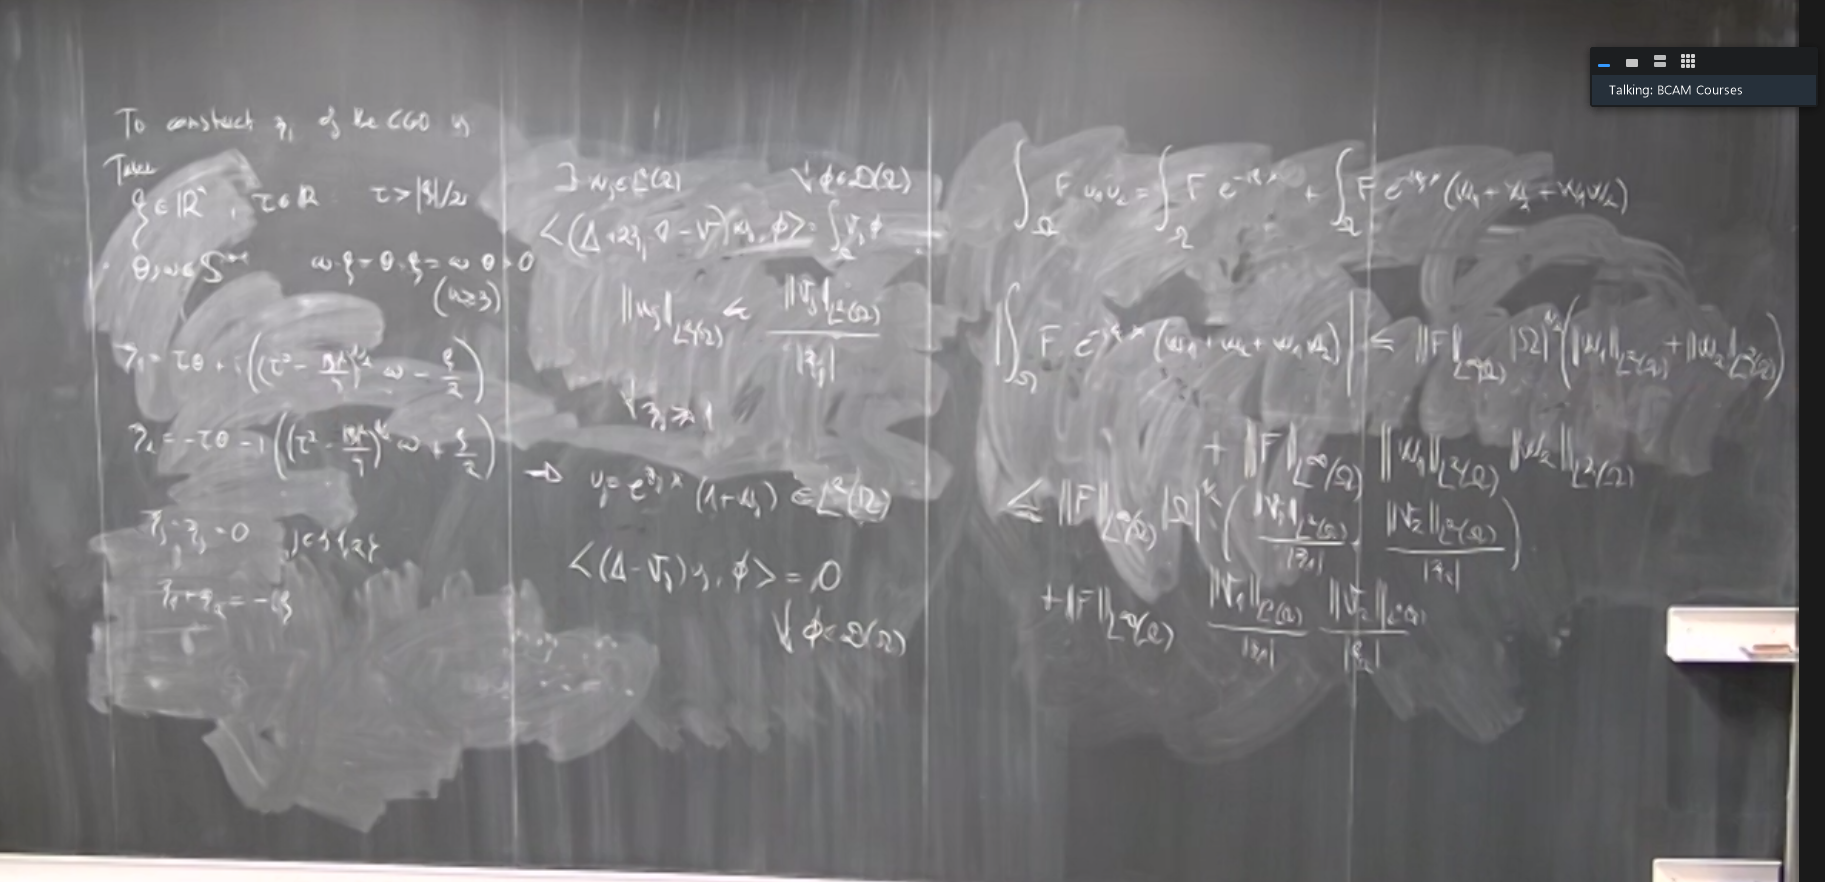
\includegraphics[width=\textwidth]{screenshots/1.png}

    \item That means that:
    \begin{equation}
        \lim_{\zeta \rightarrow \infty} |\int_\Omega F e^{-i\zeta \cdot x} (\omega_1 + \omega_2 + \omega_1\omega_2)| = 0  \implies  \int_\Omega F e^{-i\zeta \cdot x} = 0  \implies  \hat{F}(\zeta) = 0, \ \zeta \text{ arbitrary} \implies F = 0
    \end{equation}

    \item \textbf{6. The Calderón Problem Uniqueness:} $\Omega$ is a bounded open subsut of $\mathbf{R}^n$ with $ n\geq 3$.
    \begin{equation}
        \Lambda_\gamma \in \mathcal{L}(H^1(\Omega)/H^1_0(\Omega), (H^1(\Omega)/H^1_0(\Omega))^*) \text{ is self-adjoint}
    \end{equation}
    \begin{equation}
        \langle \Lambda_\gamma  f, g \rangle = \int \gamma \nabla v \cdot \nabla u
    \end{equation}
    \begin{equation}
        \forall f, g \in H^1(\Omega)/H^1_0(\Omega)
    \end{equation}
    \begin{equation}
        u \in H^1(\Omega): \text{tr} [u] = f, \ \int_\Omega \gamma \nabla u \cdot \nabla \phi = 0 \ \forall \phi \in \mathcal{D}(\Omega)
    \end{equation}
    \begin{equation}
         v \in H^1(\Omega): \text{tr} [v] = g
    \end{equation}
    \begin{equation}
        \langle \Lambda_\gamma  g, f \rangle = \int_\Omega \gamma \nabla u \cdot \nabla v = \langle \Lambda_\gamma  f, g \rangle \ \text{so it's self-adjoint}
    \end{equation}

    \item \textbf{6.1. From the boundary to the interior:} We are going to see that:
    \begin{equation}
        \Lambda_{\gamma_1} - \Lambda_{\gamma_2} \rightarrow \int_\Omega (\gamma_1 - \gamma_2) \nabla u \cdot \nabla v = 0
    \end{equation}
    \begin{equation}
        \forall u_j  \in H^1_0(\Omega). \ \int_\Omega \gamma_j \nabla u_j \cdot \nabla \phi = 0 \ \forall \phi \in \mathcal{D}(\Omega)
    \end{equation}

    \item Take $f_1, f_2 \in H^1(\Omega)/H^1_0(\Omega$ and by the direct problem  we know $\exists! u_1, u_2\in H^1(\Omega): \ \int_\Omega \gamma_j \nabla u_j \cdot \nabla \phi \ \forall \phi \in \mathcal{D}(\Omega)$ where $\text{tr} [u_j] = f_j$:
    \begin{equation}
        \langle \Lambda_{\gamma_1} f_1, f_2 \rangle = \int_\Omega \gamma_1 \nabla u_1 \cdot \nabla u_2
    \end{equation}
    \begin{equation}
        \langle \Lambda_{\gamma_2} f_2, f_1 \rangle = \int_\Omega \gamma_2 \nabla u_1 \cdot \nabla u_2
    \end{equation}
    and, using self-adjointness in the second equality,
    \begin{equation}
        \int_\Omega (\gamma_1 - \gamma_2) \nabla u_1 \cdot \nabla u_2 = \langle \Lambda_{\gamma_1} f_1, f_2 \rangle - \langle \Lambda_{\gamma_1} f_2, f_1 \rangle =  \langle \Lambda_{\gamma_1} f_1, f_2 \rangle - \langle \Lambda_{\gamma_2} f_1, f_2 \rangle = \langle (\Lambda_{\gamma_1} - \Lambda_{\gamma_2}) f_1, f_2 \rangle
    \end{equation}
    Then
    \begin{equation}
        \Lambda_{\gamma_1} = \Lambda_{\gamma_2} \implies \int_\Omega (\gamma_1 - \gamma_2) \nabla u_1 \cdot \nabla u_2 = 0 \ \text{is now proved(?)}
    \end{equation}

    \item Remember: $L \in L^\infty$.

    \item How do you go from here to there? Philosophical interpretration?
    \begin{equation}
        \int_\Omega (\gamma_1 - \gamma_2) \nabla u_1 \cdot \nabla u_2 \longrightarrow \int_\Omega F u_1 u_2
    \end{equation}

    \item Remember: $\gamma$ never vanishes.

    \item Try this:
    \begin{equation}
        \nabla \cdot(\gamma \nabla u) = 0 \rightarrow \gamma \Delta u + \nabla \gamma \cdot \nabla u = 0 \rightarrow \Delta u + \gamma^{-1} \nabla \gamma \cdot \nabla u =0 \rightarrow (\Delta + \gamma^{-1} \nabla \gamma \cdot \nabla) u = 0
    \end{equation}

    \item Now he does a change of variables (like in ODEs) to obtain the desired form (but I was distracted and did not follow/copy :().

    \item Liouville's transformation:
    \begin{equation}
        x'' + bx' = 0 \rightarrow y'' + cy = 0
    \end{equation}
    \begin{equation}
        x = e^\phi y \quad \text{or} \quad u = e^\phi v
    \end{equation}
    \begin{equation}
        b \rightarrow \gamma^{-1} \nabla \gamma = \nabla \log \gamma
    \end{equation}
    \begin{equation}
        \phi \rightarrow - \frac{1}{2} \log \gamma
    \end{equation}
    \begin{equation}
        \phi' \rightarrow - \frac{1}{2}\nabla \log \gamma
    \end{equation}

    \item We obtain:
    \begin{equation}
        \Delta v - \gamma^{-1/2} \Delta \gamma^{1/2} v  = 0
    \end{equation}
\end{itemize}


\section*{Day 7}
\begin{itemize}
    \item Liouville's tranformation:
    \begin{equation}
        \nabla \cdot (\gamma \nabla u) = 0 \iff \Delta u + \nabla \log (\gamma) \cdot \nabla u = 0 \iff \Delta v - \underbrace{\gamma^{-1/2} \Delta \gamma^{1/2} v }_{V} = 0
    \end{equation}
    
    \item If we plug these type of solutions in the original problem, problems will arise related to the gradients(?).

    \item \textbf{Second orthogonal relation (formal)}: 
    \begin{equation}
        \int_\Omega (V_1 - V_2) v_1 v_2 = \int_\Omega [\Delta v_1 v_2 - v_1 \Delta v_2 ] = \int_{\partial\Omega} [ \partial_\nu v_1 v_2 - v_1 \partial_\nu v_2] = 
    \end{equation}
    \begin{equation}
        = \int_{\partial\Omega} [ (\gamma_1^{1/2} \partial_\nu v_1 + v_1 \partial_ \nu\gamma_2^{1/2}) \gamma_2^{1/2} u_2 - \gamma_1^{1/2} u_1 (\gamma_2^{1/2} \partial_\nu v_2 + v_2 \partial_ \nu\gamma_1^{1/2})] = 
    \end{equation}
    where, in the first equality, we have used that $v_j$ is a solution of $(\Delta - V_j)v_j = 0$: and $\partial_\nu$ is the normal derivative. Do the derivatives and try to cancel.

    \item Let's assume that (you can in fact prove it, but we will just assume for our humble purposes):
    \begin{equation}
        \gamma_1|_{\partial\Omega} = \gamma_2|_{\partial\Omega}
    \end{equation}
        \begin{equation}
        \partial_\nu\gamma_1|_{\partial\Omega} = \partial_\nu\gamma_2|_{\partial\Omega}
    \end{equation}
    \begin{equation}
        = \int_{\partial\Omega} [\gamma_1 \partial_\nu u_1 u_2 - u_1 \gamma_2 \partial_\nu  u_2] = \int_{\partial\Omega} [\Lambda_{\gamma_1}(u_1|_{\partial\Omega}) u_2 - u_1 \Lambda_{\gamma_2}(u_2|_{\partial\Omega}) ] = \int_{\partial\Omega} (\Lambda_{\gamma_1}- \Lambda_{\gamma_2}) (u_1|_{\partial\Omega}) u_2
    \end{equation}

    \item So, formally, we have:
    \begin{equation}
        \Lambda_{\gamma_1} = \Lambda_{\gamma_2} \implies \int_\Omega (V_1 - V_2)v_1v_2 = 0 \quad \forall v_j: \ \Delta v_j - V_j v_j = 0 \ \text{in} \ \Omega
    \end{equation}
    with $V_j = \gamma_j^{1/2} \Delta \gamma_j^{1/2}$.

    \item Spaces where things belong:
    \begin{equation}
        \gamma_j \in W^{2, \infty}(\Omega)
    \end{equation}
    \begin{equation}
        \text{If } v_j \in H^1(\Omega) \implies u_j \in H^1(\Omega)
    \end{equation}

    \item \textbf{Proof of Liouville's transformation}:
    \begin{equation}
        u \in H^1(\Omega): \quad \int_\Omega \gamma \nabla u \cdot \nabla \phi = 0 \quad \forall \phi \in H_0^1
    \end{equation}
    \begin{equation}
        \gamma \in W^{?,?}
    \end{equation}
    \begin{equation}
        |\gamma^{-1} ([\gamma_0, \gamma^0])| = |\Omega|
    \end{equation}
    \begin{equation}
        v = \gamma^{1/2} u
    \end{equation}
    \begin{equation}
        \psi = \gamma^{1/2} \phi
    \end{equation}

    \item Let's see the equations these satisfy:
    \begin{equation}
        \int_{\Omega} \gamma \nabla (\gamma^{1/2} v) \cdot \nabla (\gamma^{1/2} \psi) = \int_\Omega \gamma [\gamma^{1/2} \nabla v + v \nabla \gamma^{1/2}] \cdot [\gamma^{1/2} \nabla \psi + \psi \nabla \gamma^{1/2}] = 
    \end{equation}
    \begin{equation}
        = \int_\Omega \nabla u \cdot \nabla \psi + \gamma^{1/2} \nabla v \cdot \gamma^{-1/2} \psi + \gamma^{1/2} \nabla \psi \cdot \nabla \gamma^{-1/2} v + \nabla \gamma^{1/2} \cdot \nabla \gamma^{1/2} v \psi =
    \end{equation}
    use that $\nabla (\gamma^{1/2} \gamma^{-1/2}) = 0$,
    \begin{equation}
        = \int_\Omega [\nabla v \cdot \nabla \psi - \gamma^{1/2} \nabla \gamma^{1/2} [\nabla v \psi + v \nabla \psi] - \gamma^{- 1/2} \nabla \gamma^{1/2} + \gamma^{1/2} \nabla \gamma^{1/2} v \psi] = 
    \end{equation}
    \begin{equation}
        = \int_\Omega [\nabla u \cdot \nabla \psi - \gamma^{1/2} \nabla \gamma^{1/2} \cdot \nabla (u\psi) - \nabla \gamma^{1/2} \cdot \nabla \gamma^{1/2} v \psi]=
    \end{equation}
    \begin{equation}
        = \int_\Omega \underbrace{[\nabla u \cdot \nabla \psi - \nabla \gamma^{1/2} \cdot \nabla (\gamma^{-1/2} v \psi)]}_{\text{This is fine, the above Idk}}
    \end{equation}

    \item \textbf{Proposition (Alessandrini orthogonal identity, 1988)}: $\gamma_1, \gamma_2 \in W^{2, \infty}(\Omega)$ such that $|\gamma_j^{-1}([\gamma_0, \gamma^0]) |  = |\Omega|$, $\Omega$ is open bounded and $\partial \Omega$ is Lipschitz:
    \begin{equation}\label{first-integral-formula}
        \Lambda_{\gamma_1}= \Lambda_{\gamma_2} \implies \int_\Omega (V_1 - V_2 )v_1 v_2 = 0
    \end{equation}
    whenever
    \begin{equation}
        \int_\Omega [\nabla u \cdot \nabla \psi - \nabla \gamma^{1/2} \cdot \nabla (\gamma^{-1/2} v \psi)] = 0
    \end{equation}
    with $V_j = \gamma^{1/2} \Delta \gamma^{1/2}$.

    \item \textbf{Proof (Alessandrini's)}:
    \begin{itemize}
        \item We have the following:
        \begin{equation}
            W_0^{2, \infty} = \overline{\mathcal{D}(\Omega)}^{|| \cdot ||_{W^{2, \infty}}}
        \end{equation}
        \begin{equation}
            || \cdot ||_{W^{2, \infty}} = \sum_\alpha ||\partial^\alpha||_{L^\infty}
        \end{equation}
        \item Use \textit{first integral formula} (\ref{first-integral-formula}):
        \begin{equation}
            0 = \int_\Omega \gamma_j \nabla v_j \cdot \nabla v_k = \int_\Omega \gamma_j \nabla (\gamma^{1/2}_j v_j) \cdot \nabla (\gamma^{-1/2}_k v_k) =  
        \end{equation}
        \begin{equation}
            = \int_\Omega \gamma_j \nabla (\gamma^{1/2}_j v_j)\cdot \nabla (\gamma^{-1/2} v_k) + \underbrace{\int_\Omega \gamma_j \nabla (\gamma^{1/2}_j v_j)\cdot \nabla(\gamma^{-1/2}_k - \gamma^{-1/2}_j) v_k) }_{0} =
        \end{equation}
        \begin{equation}
            (\gamma^{-1/2}_k - \gamma^{1/2}_j) v_k \in H_0^1(\Omega)
        \end{equation}

        \item The following can be approximated by functions in $C^\infty(\Omega)$ (check Evan's book):
        \begin{equation}
            v_k \in H^1(\Omega)
        \end{equation}

        \item Do the same computations as we did in Liouville's:
        \begin{equation}
            = \int_\Omega [\nabla v_j \cdot \nabla v_k - \nabla \gamma^{1/2}_j \cdot \nabla (\gamma^{-1/2} v_j v_k)]
        \end{equation}
        
        \item Then we have (this will be in the future our \textit{orthogonality relation}):
        \begin{equation}
            \Lambda_{\gamma_1} = \Lambda_{\gamma_2} \implies 0 = \int_\Omega (\gamma_1 - \gamma_2) \nabla u_1 \cdot \nabla u_2 = \int_\Omega \nabla \gamma^{1/2}_2 \cdot \nabla (\gamma^{1/2}_2 v_1 v_2) - \int_\Omega \nabla \gamma^{1/2}_1 \cdot \nabla (\gamma^{1/2}_1 v_1 v_2)
        \end{equation}
        \begin{equation}
            = \int_\Omega \nabla (\gamma^{1/2}_2 - \gamma^{1/2}_1) \cdot \nabla(\gamma^{-1/2} v_1 v_2) - \int_\Omega \nabla \gamma^{1/2}_1 \cdot \nabla (\gamma^{1/2}_1 - \gamma^{-1/2}_1)v_1v_2) = 
        \end{equation}

        \item And now we can integrate by parts in the \textit{weak} sense:
        \begin{equation}
            \gamma^{\pm 1/2}_1 - \gamma^{\pm1/2}_2 \in H_0^1(\Omega)
        \end{equation}
        \begin{equation}
            = - \int_\Omega \Delta(\gamma^{1/2}_2 - \gamma^{1/2}_1) \gamma^{1/2}_2 v_1v_2 - \int_\Omega \Delta \gamma^{1/2} \cdot (\gamma^{1/2}_2 - \gamma^{-1/2}_1) v_1v_2 = \int_\Omega (V_1 - V_2) v_1 v_2
        \end{equation}
        and that proves the formula.
    \end{itemize}
\end{itemize}


\section*{Day 8}
\begin{itemize}
    \item \textbf{Second integral formula ($C^2$ form)}: $\Omega$ bounded open subset of $\mathbf{R}^n$, with $n>2$(?), $\partial\Omega$ of $C^1$ class, $\gamma_i \in C^2(\overline{\Omega})$ such that:
    \begin{equation}
        \partial^\alpha \gamma_1 |_\Omega = \partial^\alpha \gamma_2 |_\Omega
    \end{equation}
    \begin{equation}
        \Lambda_{\gamma_1} = \Lambda_{\gamma_2} \implies \underbrace{\int (V_1 - V_2) v_1v_2 = 0}_{\text{Second toy model}}
    \end{equation}
    whenever $v_j \in H^1$ satisfies:
    \begin{equation}
        \int_\Omega [\nabla v_1 \cdot \nabla \psi - V_j v_j \psi] = 0 \quad \forall \psi \in H^1_0(\Omega)
    \end{equation}

    \item \textbf{6.2:} We are going to prove(?):
    \begin{equation}
        \Lambda_{\gamma_1} = \Lambda_{\gamma_2} \implies V_1 = V_2
    \end{equation}
    \begin{equation}
        (\Delta v - Vv) = 0 \quad \text{where} \ v \in L^2(\Omega), V \in L^\infty(\Omega) \implies \Delta v \in L^2(\Omega)
    \end{equation}
    \begin{equation}
        \implies \partial^\alpha v|_{\Omega'} \in L^2(\Omega), \ \forall \Omega' \subset \subset \Omega
    \end{equation}
    Can we assure that $v \in H^1(\Omega)$? The answer is \textbf{no} but there is hope.

    \item The following is an argument based on the Fourier transform:
    \begin{equation}
        v \in L^2(\mathbf{R}^n), \Delta v \in L^2(\mathbf{R}^n)
    \end{equation}
    \begin{equation}
        \int_{\mathbf{R}^n} |\hat{v}(\xi)|^2 d\xi + \int_{\mathbf{R}^n} |???|^2 d\xi =  \int_{\mathbf{R}^n} ( 1 + |\xi|^4) |\hat{v}(\xi)|^2 d\xi \geq 2 \int_{\mathbf{R}^n} |\xi|^2 |\hat{v}(\xi)|^2 = ... = 2 ||\nabla v||_{L^2(\mathbf{R}^n)}
    \end{equation}

    \item Let's prove the inequality used above:
    \begin{equation}
        \exists C> 0: \forall \chi \in \mathcal{D}(\Omega), \forall v \in C^\infty(\overline{\Omega}):
    \end{equation}
    \begin{equation}
        || \chi \nabla v ||_{L^2} < C(||\chi||_{L^2} ||\Delta v||_{L^2} + ||\chi||_{W^{1, \infty}}||v||_{L^2})
    \end{equation}
    \begin{equation}
        v \in L^2, \ \Delta v \in L^? (\Omega), \ \text{and } \partial\Omega \text{ of class } C^1 
    \end{equation}
    Then $v$ can be approximated by functions in $C^\infty(\Omega)$.

    \begin{center}
        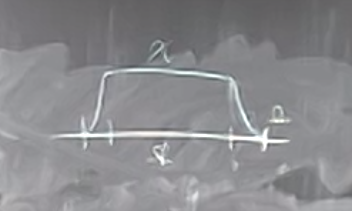
\includegraphics[width=6cm]{screenshots/2.png}    
    \end{center}
    

    \item Proof of the inequality:
    \begin{equation}
        \int_\Omega |\chi \nabla v|^2 = \int_\Omega  \chi^2 \nabla v \overline{\nabla v} = \int_\Omega 2\chi\nabla \chi\nabla v \overline{v} + \int_\Omega \chi^2 \Delta v \overline{v} 
    \end{equation}
    \begin{equation}
        |\int_\Omega \chi^2 \Delta v \overline{v} | \leq ||\chi||_{L^\infty}^2 ||\Delta v||_{L^2}||v||_{L^2} \leq ||\chi||_{L^\infty}^2 (||\Delta v||_{L^2} + ||v||_{L^2})
    \end{equation}
    \begin{equation}
        |\int_\Omega 2 \chi \nabla \chi \nabla v \overline{v}| \leq 2 ||\chi \nabla v ||_{L^2} ||\nabla \chi v||_{L^2} \leq \frac{1}{2} ||\chi \nabla v||_{L^2} + 2 ||\nabla \chi||_{L^2} ||v||_{L^2}
    \end{equation}
    where we have used $2 \frac{a}{2} b \leq \frac{1}{2}a^2 + 2b^2$.

    \item Choose $\Tilde{\Omega}$ bounded open, $\partial \Tilde{\Omega}$ in $C^1$ such that $\overline{\Omega} \subset \Tilde{\Omega}$:
    \begin{equation}
        \Tilde{V_j} = v_j \ \text{in } \Omega, \text{ and } 0 \text{ in } \Tilde{\Omega}\backslash \overline{\Omega}
    \end{equation}
    You construct the following
    \begin{equation}
        v = e^{\xi x} (1 + \omega)
    \end{equation}
    which is solution of the problem
    \begin{equation}
        (\Delta - \Tilde{V_j})v_j = 0 \text{ in } \Tilde{\Omega } \implies v_j|_\Omega \in H^1(\Omega)
    \end{equation}

    \item \textbf{6.3.} Using the scheme for the second toy model we deduce
    \begin{equation}
        \Lambda_{\gamma_1} = \Lambda_{\gamma_2} \implies V_1 = V_2 \implies \gamma_1 = \gamma_2
    \end{equation}
    If the following equation had uniqueness, it would be true that the $\gamma$'s would be the same.
    \begin{equation}
        \Delta (\gamma_1^{1/2} - \gamma_2^{1/2}) - \gamma_1^{1/2} \Delta \gamma_2^{1/2}(\gamma_1^{1/2} - \gamma_2^{1/2}) = 0
    \end{equation}
    \begin{equation}
        \gamma_1^{1/2} = \gamma_2^{1/2}?
    \end{equation}
    \begin{equation}
        v = (\gamma_1^{1/2} - \gamma_2^{1/2})
    \end{equation}
    \begin{equation}
        V = \gamma_2^{1/2} \Delta \gamma_2^{1/2}
    \end{equation}
    If we call
    \begin{equation}
        u = \gamma_2^{-1/2} v
    \end{equation}
    and do the Liouville's transformation, by poincaré inequality we know we have uniqueness on the following:
    \begin{equation}
        \nabla \cdot (\gamma_2 \nabla u ) = 0 \implies u = 0 \implies v= 0 \implies \gamma_1 = \gamma_2
    \end{equation}

    \item \textbf{Theorem}: $\Omega$ bounded open subset of $\mathbf{R}^n$, $n\geq3$, $\partial \Omega$ is of $C^1$ class, $\gamma_1, \gamma_2 \in C^2(\overline{\Omega})$:
    \begin{equation}
        \gamma_0 \leq \gamma_j \leq \gamma^0
    \end{equation}
    \begin{equation}
        \partial^\alpha \gamma_1|_{\partial \Omega} = \partial^\alpha \gamma_2|_{\partial \Omega}
    \end{equation}
    and I am missing a couple of lines here (the Zoom video just finished).
\end{itemize}



\section*{Day 9}

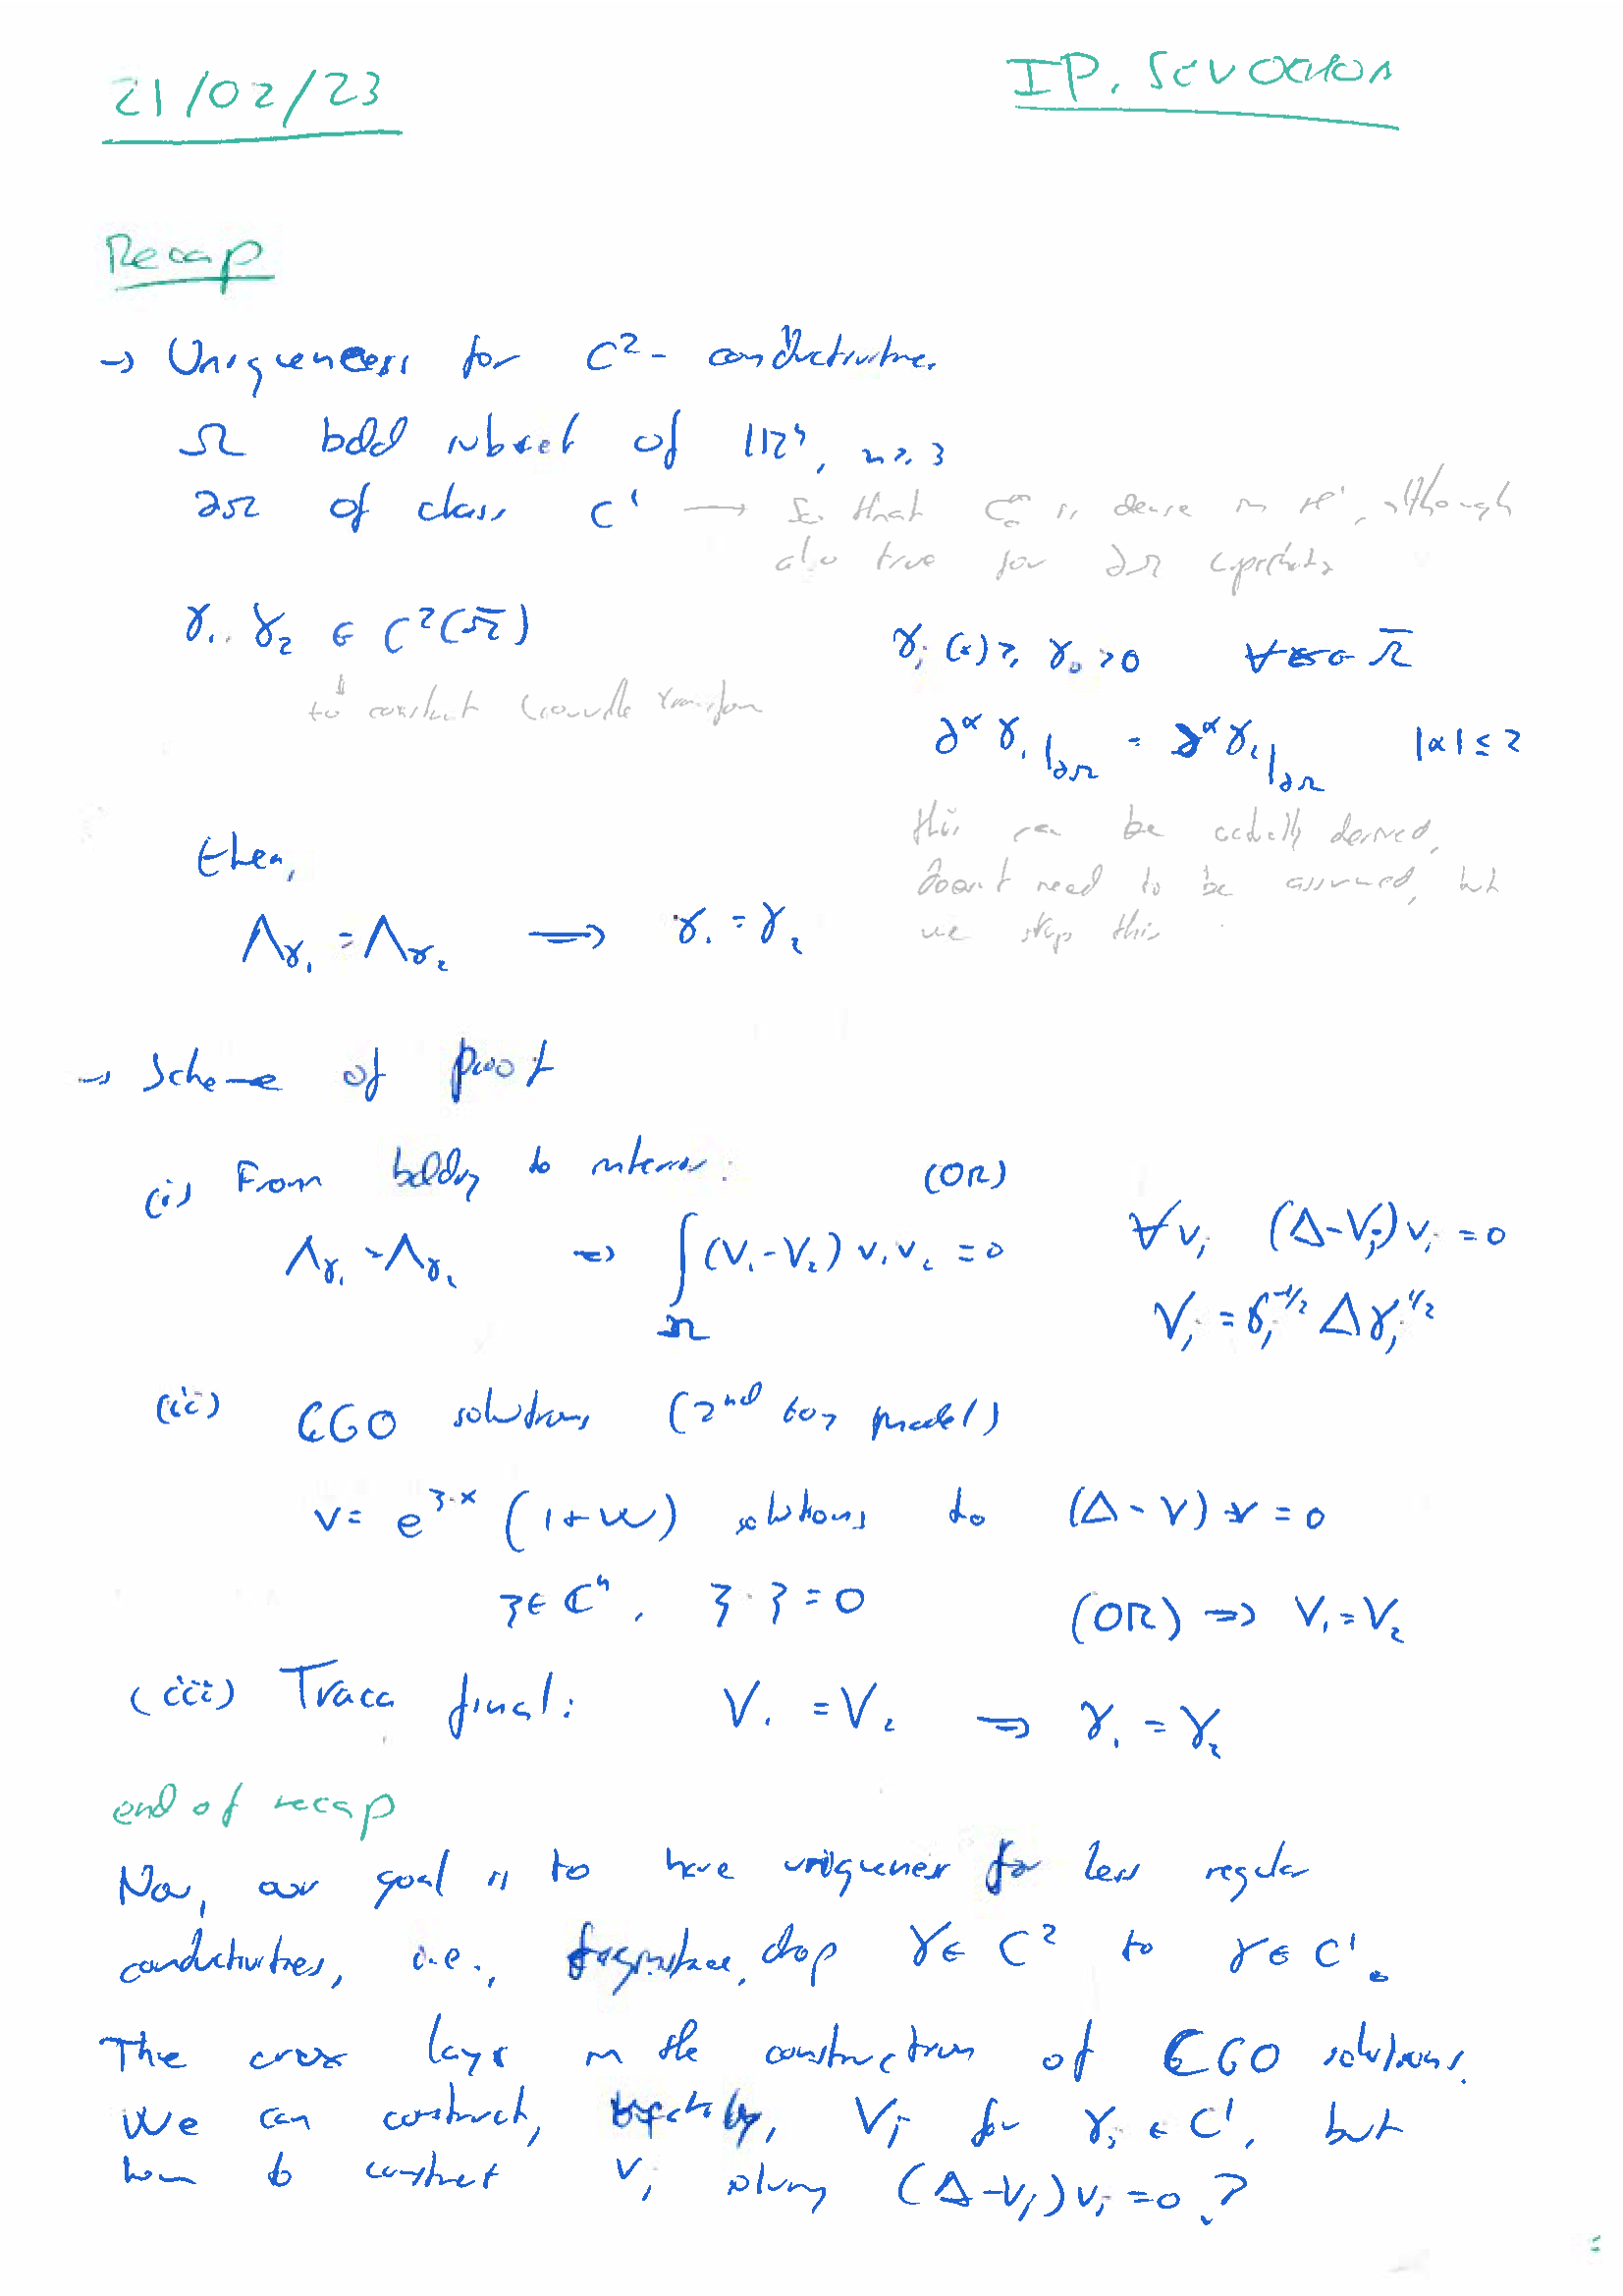
\includegraphics[width=\textwidth]{screenshots/3.png}

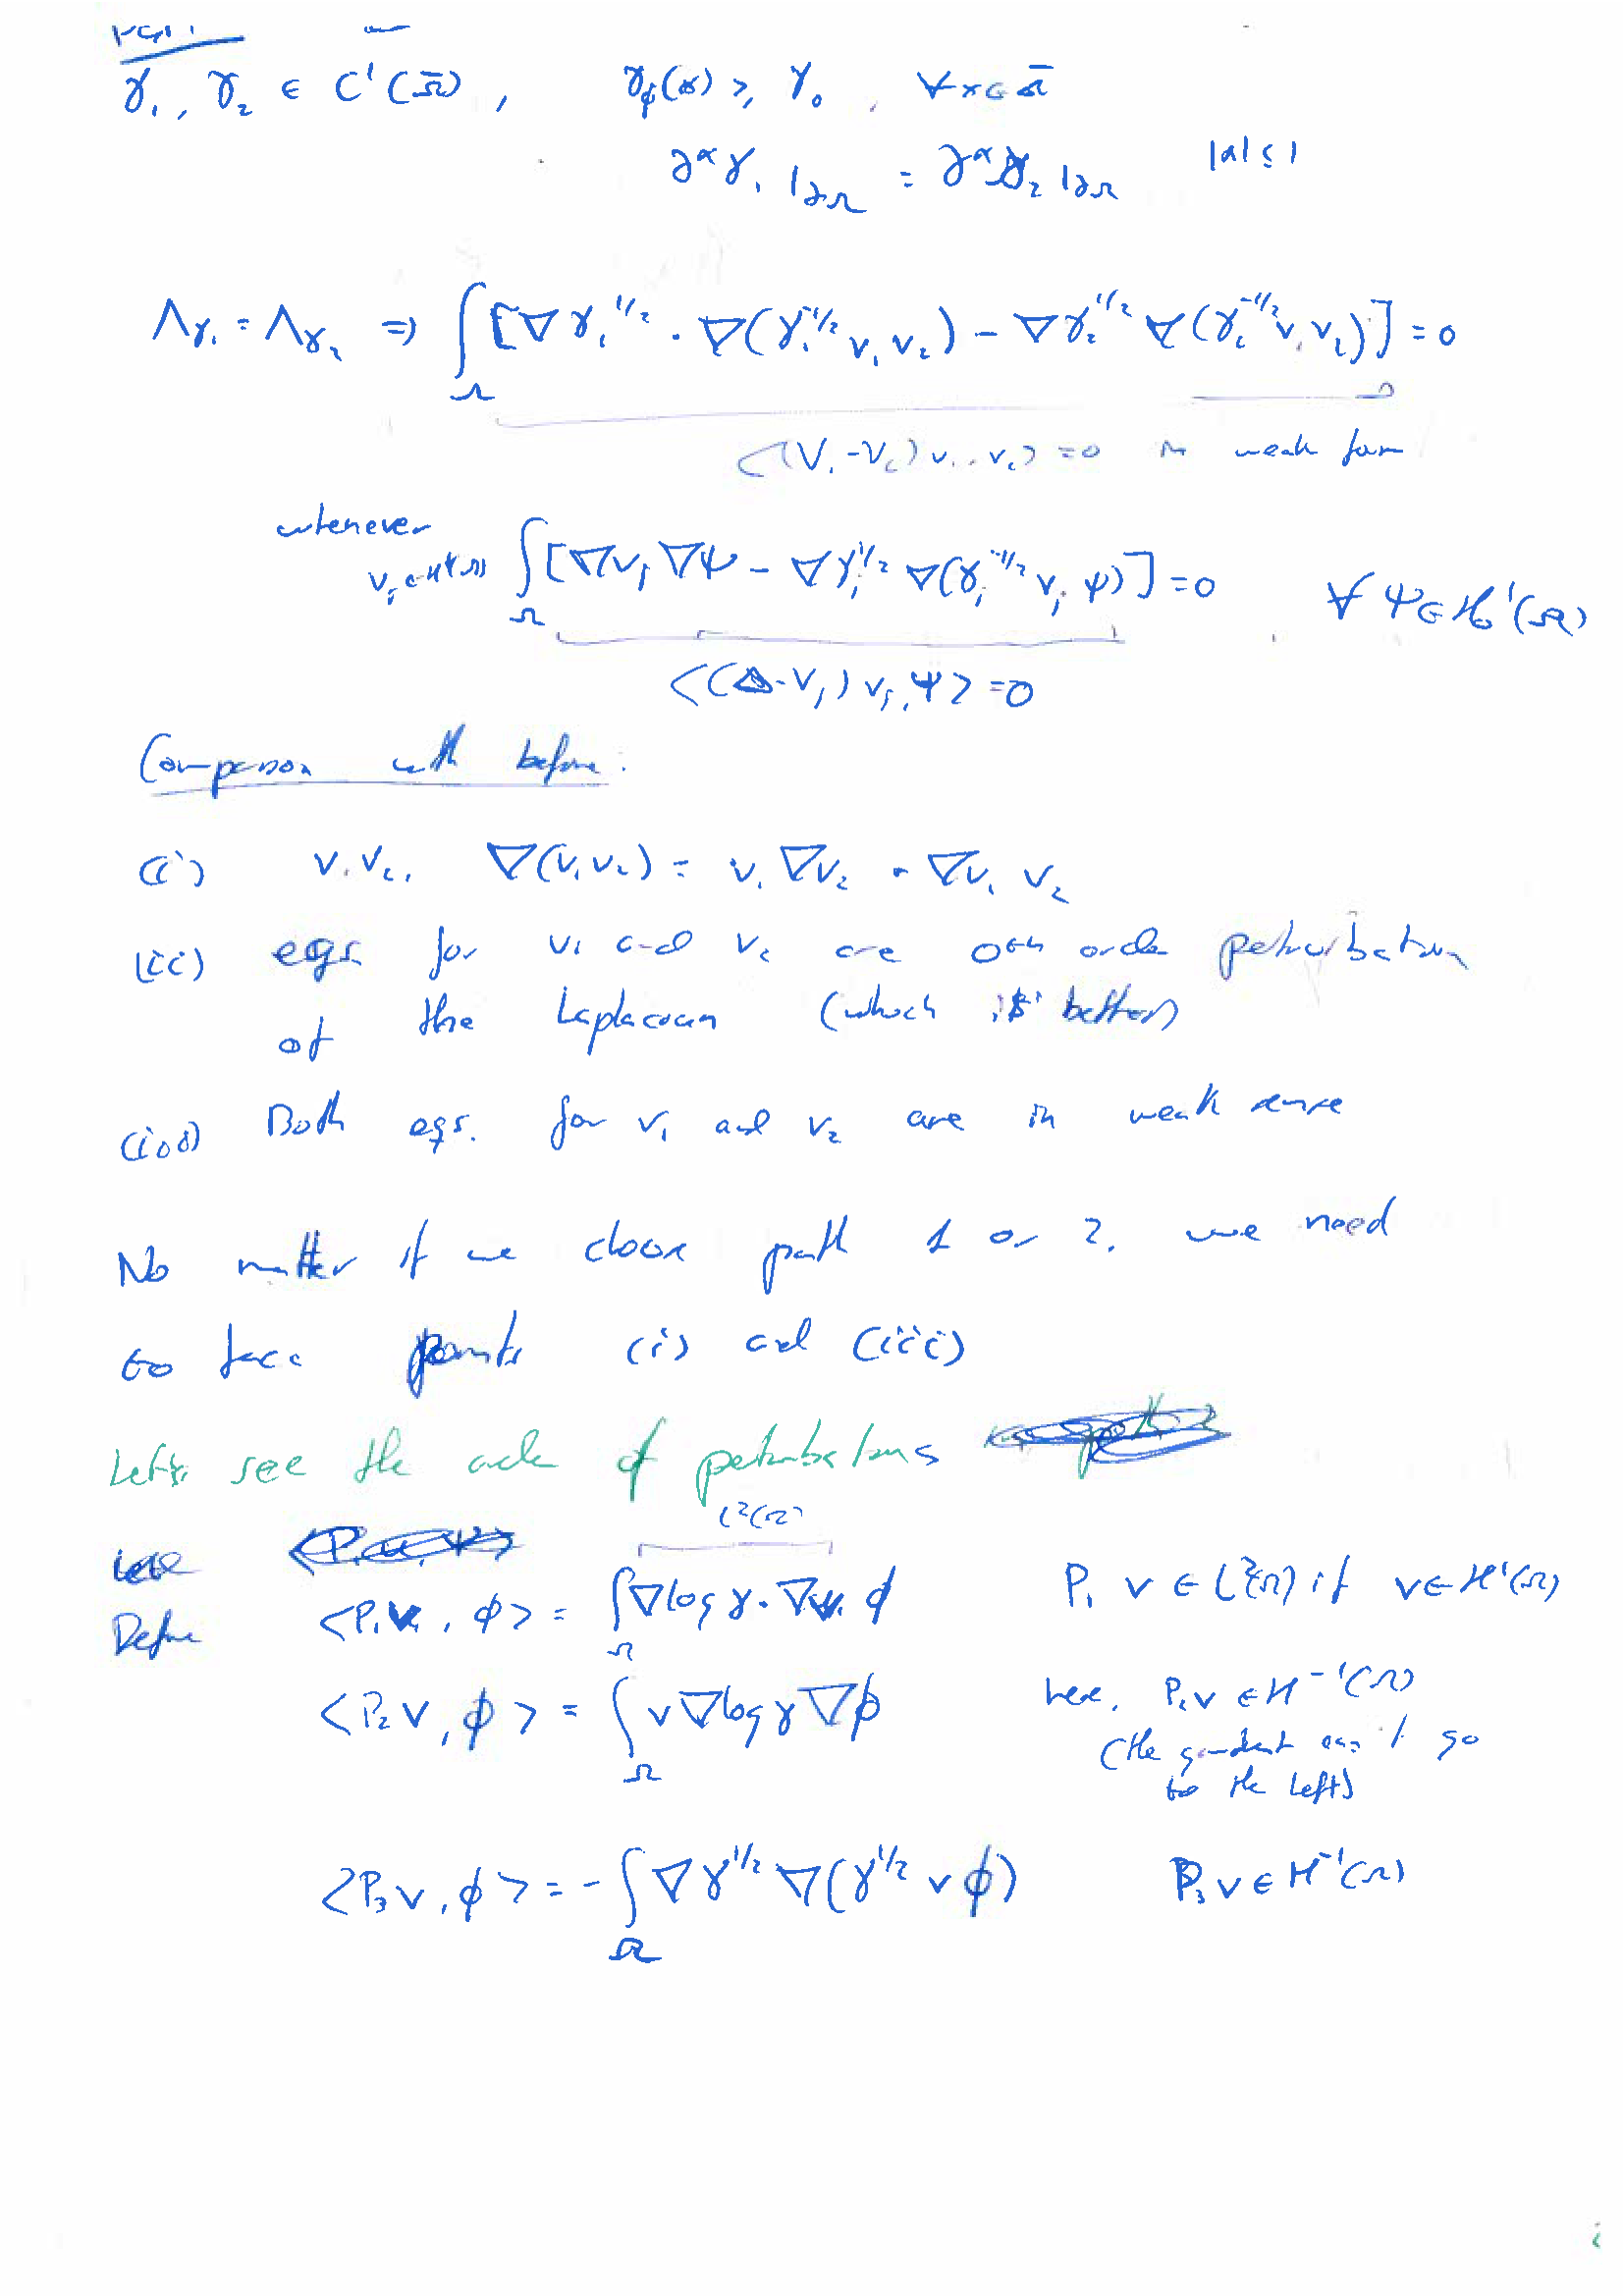
\includegraphics[width=\textwidth]{screenshots/4.png}


\section*{Day 10}
\begin{itemize}
    \item \textbf{7.1. Scheme of the proof for less regular conductivities}
    \begin{equation}
        v_k = e^{\zeta_j \cdot x} (1 + \omega_j) 
    \end{equation}
    \begin{equation}
        \zeta_j \in \mathbf{C}^n, \ \zeta_j \cdot \zeta = 0, \ \zeta_1 + \zeta_2 = i\xi
    \end{equation}
    \begin{equation}
        \int_\Omega \nabla \gamma^{1/2}_j \cdot \nabla (\gamma^{-1/2}_j v_1 v_2) = \underbrace{\int_\Omega \nabla \gamma^{1/2}_j \cdot \nabla (\gamma^{-1/2}_j e^{-i\xi \cdot x})}_{\text{I1: Fourier Transform from here}}
        + \underbrace{\int_\Omega  \nabla \gamma^{1/2}_j \cdot \nabla ( \gamma^{-1/2}_j e^{-\xi \cdot x} (\omega_1 + \omega_2 + \omega_1 \omega_2))}_{\text{I2: Decay from here}}
    \end{equation}

    \item The second integral:
    \begin{equation}
        I_2 = \frac{1}{2} \int_\Omega  \nabla \log\gamma_j \cdot \nabla ( e^{-\xi \cdot x} (\omega_1 + \omega_2 + \omega_1 \omega_2))
        - \frac{1}{4} \int_\Omega |\nabla \log \gamma_j |^2 e^{-i\xi \cdot x} (\omega_1 + \omega_2 + \omega_1 \omega_2)
    \end{equation}
    and taking the limit when $|\xi| \rightarrow 0$:
    \begin{equation}
        || \omega_j ||_{L^2} \rightarrow 0
    \end{equation}
    \begin{equation}
        || \nabla \omega_j ||_{L^2} \rightarrow 0
    \end{equation}
    \begin{equation}
        || \omega_j \nabla \omega_k||_{L^1?} \rightarrow 0
    \end{equation}

    \item Check out the different types of distributions in $\mathbf{R}^n$: ???, ???, and functions with compact support.
    \begin{equation}
        \mathcal{D}(\mathbf{R}^n) \hookleftarrow \mathcal{S}(\mathbf{R}^n) \hookleftarrow \mathcal{E}(\mathbf{R}^n)
    \end{equation}
    and, particularly, the dual of the $C^\infty$ is $\mathcal{E}$. \color{red} Am I missing a prime as in $\mathcal{D}'$? \color{black}

    \item So:
    \begin{equation}
        V_j \in \mathcal{D}(\mathbf{R}^n)
    \end{equation}
    \begin{equation}
        \langle V_j , \phi \rangle = \int_\Omega \nabla \gamma^{1/2}_j \cdot \nabla (\gamma^{-1/2}_j \phi) \quad \forall \phi \in \mathcal{D}(\mathbf{R}^n)
    \end{equation}
    where $\text{supp} V_j \subset \overline{\Omega}$ and $V_j \in \mathcal{E}(\mathbf{R}^n)$.

    \item Particularly $\forall \psi \in H_0^1(\Omega)$:
    \begin{equation}
        \langle (V_1 - V_2, \phi \rangle = 0 \quad \forall \phi \in C_c^\infty (\Omega)
    \end{equation}
    \begin{equation}
        0 = \int_\Omega [\nabla (\gamma^{1/2}_2 - \gamma^{1/2}_1) \cdot \nabla (\gamma^{-1/2}_2 \phi) - \nabla \gamma^{1/2}_1 \cdot \nabla ((\gamma^{1/2}_1 - \gamma^{-1/2}_2) \phi)] =
    \end{equation}
    \begin{equation}
        \rightarrow \psi = \gamma^{-1/2}_2 \phi \in H_0^1, \quad \phi = \gamma^{1/2}_2 \psi
    \end{equation}
    \begin{equation}
        = \int_\Omega [\nabla (\gamma^{1/2}_{1?} - \gamma^{1/2}_{2?}) \cdot \nabla \psi - \gamma^{-1/2}_{1} \nabla \gamma^{1/2}_1 \cdot  \nabla (\gamma^{1/2}_1 - \gamma^{-1/2}_2)\psi] = \langle \Delta u, \psi \rangle - \int_\Omega \gamma^{1/2}_1 \nabla \gamma^{1/2}_{1} \cdot \nabla u  
    \end{equation}
    \begin{equation}
        \rightarrow u = \gamma^{1/2}_1 \gamma^{-1/2}_2
    \end{equation}
    \begin{equation}
        \boxed{(\Delta + \nabla \log \gamma^{1/2}_1 \cdot \nabla ) u = 0}
    \end{equation}
    \begin{equation}
        \Delta u C(\overline{\Omega})
    \end{equation}
    \begin{equation}
        \nabla \cdot (\gamma \nabla u) = 0 \text{ where } u|_{\delta \Omega} = 0 \iff \Delta u + \gamma^{1/2}_1 \nabla \gamma^{1/2}_1 \cdot \nabla\psi = 0 
    \end{equation}

    \item \textbf{Proposition}: $\Omega$ is open and bounded subset of $\mathbf{R}^n$ with $n\geq 3$:
    \begin{equation}
        \gamma_1, \gamma_2 \in C^1(\overline{\Omega})
    \end{equation}
    If
    \begin{equation}
        \int_\Omega [\nabla \gamma^{1/2}_2\cdot \nabla (\gamma^{-1/2}_2 e^{-i\xi \cdot x}) - \nabla \gamma^{1/2}_1 \cdot \nabla ((\gamma^{1/2}_2 e^{-i\xi \cdot x})] = 0 \quad \forall \xi \in \mathbf{R}^n
    \end{equation}
    then
    \begin{equation}
        \gamma_1 = \gamma_2
    \end{equation}

    \item \textbf{7.2. CGO for less regular conductivities}:

    Take the following perturbation:
    \begin{equation}
        Q_\gamma : v \in H^1(\Omega) \rightarrow Q_\gamma v \in H^{-1?}(\Omega)
    \end{equation}
    \begin{equation}
        \langle Q_\gamma v, \psi \rangle = - \int_\Omega \nabla \gamma^{1/2} \cdot \nabla (\gamma^{-1/2} v \psi)
    \end{equation}
    \begin{equation}
        \langle V, \psi \rangle = \langle Q_\gamma \mathbf{1}, \psi \rangle = - \int_\Omega \nabla \gamma^{1/2} \cdot \nabla (\gamma^{-1/2} \psi) 
    \end{equation}

    \item We want to construct:
    \begin{equation}
        v \in H^1(\Omega): \ \int_\Omega \nabla u \cdot \nabla \psi + \langle Q_\gamma v, \psi \rangle = 0 \ \forall \psi \in H_0^1(\Omega)
    \end{equation}
    in the form
    \begin{equation}
        \Delta v + Q_\gamma v= 0
    \end{equation}
    \begin{equation}
        v = e^{\zeta \cdot x} (1+\omega), \ \zeta \in \mathbf{C}^n, \ \zeta \cdot \zeta = 0
    \end{equation}

    \item Take $\psi = e^{-\zeta \cdot x} \psi$.
    \begin{equation}
        \int_\Omega \nabla v \cdot \nabla (e^{-\zeta \cdot x} \phi) + \langle Q_\gamma v, \psi \rangle = 
    \end{equation}
    \begin{equation}
        = \int_\Omega (\nabla (1+\omega) + (1+\omega) \zeta) \dot (\nabla \psi - \zeta \phi) + \langle Q_\gamma (1+\omega), \phi \rangle =
    \end{equation}
    \begin{equation}
        = \int_\Omega [\nabla \omega \cdot \nabla \phi - \zeta \cdot \nabla \omega \phi +\underbrace{ (1+\omega) \zeta \cdot \nabla \phi}_{(*)}] + \langle Q_\gamma \omega, \phi \rangle + \langle V, \phi\rangle 
    \end{equation}
    \begin{equation}
        (*) = - \int_\Omega \zeta \cdot \nabla \omega \phi
    \end{equation}

    \item If 
    \begin{equation}
        \boxed{\int_\Omega \nabla \omega \cdot \nabla \phi - 2 \zeta \cdot \nabla \omega \phi + \langle Q_\gamma \omega, \phi \rangle = - \langle V, \phi \rangle \ \forall \phi \in H_0^1}
    \end{equation}
    then
    \begin{equation}
        \int_\Omega \nabla v \cdot \nabla \zeta + \langle Q_\gamma v, \psi\rangle = 0 \ \forall \psi \in H_0^1
    \end{equation}
    where $V = Q_\gamma \mathbf{1}$.

    \item \textbf{The method of a priori estimates} (again):
    \begin{equation}
        L: u \in H^1(\Omega) \rightarrow \Delta u + 2 \zeta \cdot \nabla u = Q_\gamma u \in H^{-1}(\Omega)
    \end{equation}
    with $L$ surjective.
    \begin{equation}
        \forall f \in H^{-1}, \text{ I want } \exists u \in H^1(\Omega): \ Lu = f
    \end{equation}

    \item If
    \begin{equation}
        ||\phi||_{H_0^1} \leq ||L^T \phi||_{H_0^1} \ \forall \phi \in H_0^1
    \end{equation}
    then $L$ is surjective.
    
    
\end{itemize}

\section*{Day 11}
\begin{itemize}
    \item We are going to repeat a computation due to a mistake in the last day:
    \begin{itemize}
        \item We had:
        \begin{equation}
            V_1 = V_2 \rightarrow \gamma_1 = \gamma_2 \ (\gamma_j  \in C^1(\overline{\Omega})
        \end{equation}
        \begin{equation}
            0 = \int_\Omega [\nabla \gamma^{1/2}_2 \cdot \nabla (\gamma^{-1/2}_1 \phi) - \nabla \gamma^{1/2}_1 \cdot \nabla (\gamma^{-1/2}_1 \phi) ] \ \forall \phi \in H^1_0 (\Omega)
        \end{equation}
    
        \item So now, what we would do is just add and substract the same type of terms:
        \begin{equation}
            = \int_\Omega [\nabla (\gamma^{1/2}_2 - \gamma^{1/2}_1) \cdot \nabla (\gamma^{-1/2}_1 \phi) - \nabla \gamma^{1/2}_1 \cdot \nabla ((\gamma^{-1/2}_1 - \gamma^{-1/2}_2)  \phi) ]
        \end{equation}
        and considering $\phi = \gamma_2^{1/2}\psi \in H^1_0(\Omega)$ we have
        \begin{equation}
            = \int_\Omega [\nabla (\gamma^{1/2}_2 - \gamma^{1/2}_1) \cdot \nabla \psi - \nabla \gamma^{1/2}_1 \cdot \nabla ((\frac{\gamma^{1/2}_2}{\gamma^{1/2}_1} - 1) \psi)]
        \end{equation}
        \begin{equation}
            = \int_\Omega [\nabla (\gamma^{1/2}_2 - \gamma^{1/2}_1) \cdot \nabla \psi - \nabla \gamma^{1/2}_1 \cdot \nabla (\gamma^{-1/2}_1)(\gamma^{1/2}_2 - \gamma^{1/2}_1)\psi]
        \end{equation}
    
        \item Now, call $v = \gamma^{1/2}_2 - \gamma^{1/2}_1$, and we have:
        \begin{equation}
            = - \langle \Delta v, \psi \rangle + \langle Q_{\gamma_1} v, \psi \rangle
        \end{equation}
    
        \item And if $u = \gamma^{-1/2}_1 v$, you can prove thar
        \begin{equation}
            \int \gamma_1  \nabla u \cdot \nabla \phi = 0  \ \forall \phi \in H_0^1(\Omega)
        \end{equation}
    
        \item Since
        \begin{equation}
            \gamma_1|_{\partial \Omega} = \gamma_2|_{\partial \Omega} \implies v|_{\partial \Omega} = 0 \implies u \in H^1_0(\Omega)
        \end{equation}
    
        \item All this implies that
        \begin{equation}
            u = 0 \implies v= 0 \implies \gamma_1 = \gamma_2
        \end{equation}
    \end{itemize}

    \item \textbf{Recap}: We have to show now that $v_1 = v_2$.$\Omega$ bounded domain in $\mathbf{R}^n$ with $n\geq 2$, $\partial \Omega$ of $C^1$ class, $\gamma_j \in C^1(\overline{\Omega})$ with $\partial^\alpha \gamma_1|_{\partial \Omega} = \partial^\alpha \gamma_2|_{\partial \Omega}$
    \begin{equation}\label{orthogonality-relation}
        \Lambda_{\gamma_1} = \Lambda_{\gamma_2} \implies \int_\Omega [\nabla \gamma^{1/2}_1 \cdot \nabla (\gamma^{-1/2}_1) v_1v_2 - \nabla \gamma^{1/2}_2 \cdot \nabla (\gamma^{-1/2}_2) v_1v_2] = 0
    \end{equation}
    \begin{equation}
        \forall v_j \in H^1(\Omega): \ \Delta v_j - Q_{\gamma_j} v_j = 0
    \end{equation}
    
    \item If $\omega \in H^1(\Omega)$ such that $(\Delta + 2\zeta \cdot \nabla ) \omega - Q_\gamma \omega = V$ with $\zeta \in \mathbf{C}$ such that $\zeta \cdot \zeta = 0$.
    \begin{equation}
        \implies v = e^{\zeta \cdot x} (1 + \omega) \in H^1(\Omega)
    \end{equation}

    \item Remember that we now apply the method of a priori estimates:
    \begin{equation}
        L: u \in H^1(\Omega) \rightarrow (\Delta + 2\zeta \cdot \nabla - Q_\gamma ) u \in H^{-1}(\Omega)
    \end{equation}
    Then:
    \begin{equation}\label{inequality}
        ||\phi||_{H^1(\mathbf{R}^n)} \leq ||L^T \phi||_{H^{-1}(\mathbf{R}^n)} \ \forall \phi \in C^\infty_c (\Omega)
    \end{equation}
    implies
    \begin{equation}
        \implies \forall f \in H^{-1}(\Omega), \ \exists u  \in H^1(\Omega), \ Lu = f
    \end{equation}

    \item \textbf{Remember}: to prove surjectivity of $L$, we need to prove injectivity of $L^T$ via the above inequality. "\textit{This is our goal today, and not only today}."

    \item We want to construct CGO solutions and test our orthogonality relation (Eq. (\ref{orthogonality-relation})), and for that we only need to prove inequality in Eq. (\ref{inequality}).

    \item We have the following, looking for the \textbf{key} inequality:
    \begin{equation}
        ||  (\Delta - 2\zeta \cdot \nabla) \phi ||_{L^2(\mathbf{R}^n)} \geq |\Re \zeta| || \phi ||_{L^2(\mathbf{R}^n)} + || (\Delta + 2 \Im \zeta \cdot \nabla) \phi ||_{L^2(\mathbf{R}^n)} + || \Re \zeta \cdot \nabla \phi||_{L^2(\mathbf{R}^n)}
    \end{equation}
    
    \item Last time, we threw away the last two terms because they were positive (and we could split them because they are somehow orthogonal). In fact, these 2 terms allowed us to retain the first one. Now, we are not going to throw them away, because we want to get more information. We need a second derivative to obtain it.

    \item Notice:
    \begin{equation}
        \Delta (e^{-i \Im  \zeta \cdot x} \phi) = e^{-i \Im  \zeta \cdot x} (\Delta \phi - i2 \Im \zeta \cdot \nabla \phi - |\Im \zeta|^2 \phi)
    \end{equation}
    \begin{equation}
        ||  (\Delta - i2 \Im \zeta \cdot \nabla) \phi ||_{L^2} = || (\Delta + |\Im \zeta|^2) \cdot (e^{-i \Im  \zeta \cdot x} \phi)||_{L^2} \geq || \Delta(e^{-i \Im  \zeta \cdot x} \phi)||_{L^2} - |\Im \zeta|^2 || e^{-i \Im  \zeta \cdot x} \phi ||_{L^2}
    \end{equation}
    using Greenwald(?) inequality.

    \item Can the negative part in the previous inequality be "really negative"? Maybe not.

    \item Remember that $\zeta \cdot \zeta = 0 \implies |\Re \zeta| = |\Im \zeta |$.

    \item Let us call $\tau = |\Re \zeta|$. If we divide the inequality by $2\tau$, we can manage to absorb/control the $|\Im \zeta|^2 $ term.

    \item \textbf{Definition}: 
    \begin{equation}
        ||e^{-i \Im  \zeta \cdot x} \phi ||_{H^s_\tau(\mathbf{R}^n)} = (\int_{\mathbf{R}^n} (\tau^2 + |?|^2)^s |\hat{\phi}(\xi)|^2 d\xi)^{1/2}
    \end{equation}
    where $\alpha_1 + \alpha_2  =s$.

    \item Analogously:
    \begin{equation}
        || \phi ||_{H^s_\tau(\mathbf{R}^n)} = (\int_{\mathbf{R}^n} (\tau^2 + |?|^2)^2 |\hat{\phi}(\xi + \Im \zeta)|^2 d\xi)^{1/2} = (\int_\mathbf{R}^n (\tau^2 + |\eta - \Im \zeta|^2) |\hat{\phi}(\eta)|^2 d\eta)^{1/2}
    \end{equation}
    with $\eta = \xi + \Im \zeta$.

    \item We consider:
    \begin{equation}
        \tau^2 + |\eta - \Im \zeta|^2 = \tau^2 + \eta^2 - 2 \eta \Im \zeta + \tau^2 \geq 2\tau^2 + |\eta|^2 - 2|\eta| \tau \geq (2 -\frac{1}{c}) \tau^2 + (1-c) |\eta|^2
    \end{equation}
    using the inequality $2ab \leq c a^2 + \frac{1}{c} b^2$. And choosing $c = 2/3$:
    \begin{equation}
        \tau^2 + |\eta - \Im \zeta|^2 \geq \tau^2 |\eta|^2
    \end{equation}

    \item And going back to the previous calculation, this inequality implies that:
    \begin{equation}
        ||e^{-i \Im  \zeta \cdot x} \phi ||_{H^s_\tau(\mathbf{R}^n)} \geq ||\phi||_{H_{\tau^2}^{2?} (\mathbf{R}^n)}
    \end{equation}

    \item Taking the inequality further back:
    \begin{equation}
        ||  (\Delta - i2 \Im \zeta \cdot \nabla) \phi ||_{L^2} \geq \frac{1}{\tau} ||\phi||_{H_{\tau^2}^{2} (\mathbf{R}^n)}
    \end{equation}

    \item We have/wanted to have:
    \begin{equation}
        || L^T\phi||_{H^{-1}(\mathbf{R}^n)} \geq ||\phi||_{H^1(\mathbf{R}^n)}
    \end{equation}

    \item Pedro guesses the following:
    \begin{equation}
        || L^T\phi||_{H^{-1}_\tau(\mathbf{R}^n)} \geq \frac{1}{\tau}||\phi||_{H^1_\tau(\mathbf{R}^n)}
    \end{equation}

    \item I want to show that:
    \begin{equation}
        ||  (\Delta - 2 \zeta \cdot \nabla) \phi ||_{H^{-s}_\tau(\mathbf{R}^n)} \geq \frac{1}{\tau} ||\phi||_{H_{\tau^2}^{2-s} (\mathbf{R}^n)}
    \end{equation}
    If $s=1$, it's close to what we want. We'll do it for $s$ in general. 

    \item $\chi$ is a cut-off function to be chosen, and we need to use it because it is the only way we can make this function compactly supported in a region (but we still do not know which $\chi$ we need):
    \begin{equation}
        || (\tau^2 - \Delta)(\chi(\tau^2 - \Delta)^{-3/2}) \phi||_{L^2} = ||\chi (\tau^2 - \Delta)^{-3/2})||_{H^2_\tau}
    \end{equation}

    \item In commutator notation:
    \begin{equation}
        (\tau^2 - \Delta)(\chi(\tau^2 - \Delta)^{-3/2}) \phi = \chi (\tau^2 - \Delta)^{?-3/2}\phi - [\Delta, \chi](\chi(\tau^2 - \Delta)^{-3/2}) \phi
    \end{equation}
    where
    \begin{equation}
        [\Delta, x] \psi] = \Delta (\chi \psi) - \chi \Delta \psi
    \end{equation}

    \item We have:
    \begin{equation}
        \frac{1}{\tau} || \phi ||_{H^{s-2}_\tau(\mathbf{R}^n)} = \frac{1}{\tau} ||(\tau^2 - \Delta)^{(s-2)/2} \phi||_{L^2}
    \end{equation}

    \item Add and substract to obtain (use triangle inequality):
    \begin{equation}
        \frac{1}{\tau} || \phi ||_{H^{s-2}_\tau(\mathbf{R}^n)} \leq 
    \end{equation}
    \begin{equation}
        \frac{1}{\tau} ||(\tau^2 - \Delta) (\chi(\tau^2 -\Delta)^{-3/2} \phi)||_{L^2} + || (1 - \chi)(\tau^2 - \Delta) (\tau^2 -\Delta)^{(?-3)/2} \phi||_{L^2} + ||[\Delta, \chi] (\tau^2 -\Delta)^{-3/2} \phi||_{L^2}
    \end{equation}

    \item 
    
\end{itemize}

\section*{Day 12}
\begin{itemize}
    \item \textbf{Recap}: we wanted to prove:
    \begin{equation}
        \frac{1}{|\Re \zeta |} || \phi||_{H^?} \leq || L_\zeta^T||_{H^{-1}}
    \end{equation}
    \begin{equation}
        L_\zeta = \Delta + 2 \zeta \nabla - Q_\gamma
    \end{equation}
    
    and the $H^2$-$L^2$ inequality:
    \begin{equation}
        \exists C > 0: \ \frac{C}{|\Re \zeta|} || \phi ||_{H^2} \leq || (\Delta - 2 \zeta \nabla)\phi||_{L^2}
    \end{equation}
    \begin{equation}
        \forall \zeta \in \mathbf{C}^n, \ \zeta \cdot \zeta = 0, \ |\zeta| \geq 1, \ \forall \phi \in C^\infty_c (\Omega)
    \end{equation}
    \begin{equation}
        \langle  Q_\gamma \phi, \psi \rangle = \int_\Omega \nabla \gamma^{1/2} \cdot \nabla (\gamma^{1/2} \phi \psi)
    \end{equation}
    
    \item We have proved part of the inequality(?).

    \item We have from the previous lesson:
    \begin{equation}
        ||\phi||_{(?)} \leq \tau || (\Delta - 2\zeta \cdot \nabla) (\xi (\tau^2 - \Delta)^{-3/2} \phi) ||_{L^2} + || ((?) - \xi)(\tau^2 - \Delta)^{(?)/2}\phi||_{L^2}
    \end{equation}
    \begin{equation}
        \leq \underbrace{\tau || \chi(\Delta - 2 \zeta \cdot \nabla) [(\tau^2 - \Delta)^{-(?)/2} \phi]||_{L^2} }_{(1)} +
    \end{equation}
    \begin{equation}
        +  \underbrace{\tau ||  \underbrace{[\Delta - 2 \zeta \cdot \nabla, \chi] ((\tau^2 - \Delta)^{-3/2} \phi)}_{(2^*)}  ||_{L^2}}_{(2)}+
    \end{equation}
    \begin{equation}
        + \underbrace{|| (\Lambda(?) - \chi) (\tau^2 - \Delta)^{(?)/2} \phi ||_{L^2}}_{(4)} 
    \end{equation}

 
    \begin{equation}
        (1) \leq \tau ||(\Delta - 2 \zeta \cdot \nabla)||_{H^{-?}}
    \end{equation}
    \begin{equation}
        (2^*) = (\Delta \chi + 2 \nabla \chi \cdot \nabla - 2 \zeta \cdot \nabla \chi)((\tau^2 - \Delta)^{-?/2}\phi) 
    \end{equation}
    \begin{equation}
        (2) \leq \tau || \Delta \chi (\tau^2 - \Delta)^{-3/2} \phi ||_{L^2} + \underbrace{\tau ||(\nabla \chi \cdot \nabla - \zeta \cdot \nabla \chi)(\tau^2 - \Delta)^{-3/2}\phi ||_{H_\tau^?}}_{\text{(2'): This poses problems!}}
    \end{equation}
    \begin{equation}
        \leq \tau || \phi||_{H^{-?}} + \tau || \phi||_{H^{1-s}} + \tau^2 || \phi||_{H^{-?}}
    \end{equation}
    \begin{equation}
        \leq \underbrace{\frac{\tau}{\tau^2} || \phi||_{H^{-?}}}_{\text{Vanishes}} + \frac{\tau}{\tau} || \phi||_{H^{-?}} + \frac{\tau^2}{\tau^2} || \phi||_{H^{-?}}
    \end{equation}

    \item \textbf{Lemma}:
    
    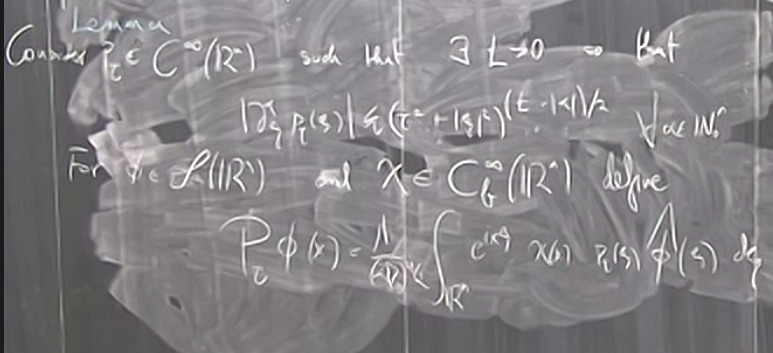
\includegraphics[width=\textwidth]{screenshots/5.png}
    
    Then
    \begin{equation}
        || P_\tau \phi ||_{L^2} \lesssim \frac{1}{\tau^N} ||\phi||_{L^2} \quad \forall \phi, \ \forall N \in \mathbf{N}
    \end{equation}

    \item We have:
    \begin{equation}
        (2') + (4) \leq \tau \underbrace{\frac{1}{\tau^N} ||\phi||_{L^2}}_{(2')} + \underbrace{\frac{1}{\tau^N} || \phi||_{L^2}}_{(4)} \leq (\frac{1}{\tau^{N-1}} + \frac{1}{\tau^N})|| \phi||_{H^{2-s}}
    \end{equation}


    \item \textbf{Proof}:
    \begin{enumerate}
        \item Write $\mathcal{P}_\tau$ in terms of the kernel.
        \begin{equation}
            \mathcal{P}_\tau \phi (x) = \frac{1}{(?)^?} \int_{\mathbf{R}^n} \chi (x) P_\tau (?)(\int_{\mathbf{R}^n}  e^{i (x -y)\cdot \zeta} \phi (y) dy) d\zeta
        \end{equation}

        \item Check which of the following expressions suits you best.
        \begin{equation}
            - \Delta_\zeta [e^{i(x -y) \cdot \zeta}] = |x - y|^2 e^{i(x -y) \cdot \zeta} \ \rightarrow \ e^{i(x -y) \cdot \zeta} = -\frac{1}{|x - y |^2} \Delta_\zeta (e^{i(x -y) \cdot \zeta})
        \end{equation}
        \begin{equation}
            (1 - \Delta_\zeta)[e^{-i(x -y) \cdot \zeta}] = (1+|x-y|^2) e^{-i(x -y) \cdot \zeta} \ \rightarrow \ e^{-i(x -y) \cdot \zeta} =  \frac{1  - \Delta_\zeta}{1 + |x - y|^2} e^{-i(x -y) \cdot \zeta}
        \end{equation}
        Careful with the singularities of the first equation. The kernel is away from the singularities in the second.

        \item The kernel can be written(?) as:
        \begin{equation}
            ??? = \int_{\mathbf{R}^n} \frac{\chi(x) \Tilde{\chi}(y)}{|x - y |^?} (\int_{\mathbf{R}^n} e^{i(x-y) \cdot \zeta} (- \Delta_\zeta)^? P_? d\zeta )\phi(y) dy = \int_{\mathbf{R}^n} \mathcal{K} (x, y) \phi (y) dy
        \end{equation}

        \item If we have the following inequality:
        \begin{equation}
            C > \sup \int_{\mathbf{R}^n}  | \mathcal{K} (x, y)| dy + \sup \int_{\mathbf{R}^n} | \mathcal{K} (x, y)| dx
        \end{equation}
        then
        \begin{equation}
            || \int_{\mathbf{R}^N} \mathcal{K} (x, y)\phi(y) dy||_{L^2} \leq \frac{1}{\tau^N} ||\phi||_{L^2}
        \end{equation}

        \item So, we have:
        \begin{equation}
            |\mathcal{K}(x,y)| \leq \frac{|\chi(x)||\Tilde{\chi}(y)|}{|x - y|^?} \int_{\mathbf{R}^N} (\tau^?)^? d\zeta
        \end{equation}
        \begin{equation}
            \rightarrow \frac{|\chi(x)||\Tilde{\chi}(y)|}{|x - y|^?} \tau^{? - 2M + ?}
        \end{equation}
    \end{enumerate}

    \item \textbf{Local vs. Pseudo-local operator}:
    \begin{itemize}
        \item \textbf{Local} meaning that $\text{supp } \mathcal{P}u \subset \text{supp } u$
        \item \textbf{Pseudo-local} meaning that $\text{sing supp } \mathcal{P}u \subset \text{sing supp } u$
    \end{itemize}
    Singular support is the support where the function is not smooth(?).

\end{itemize}

\section*{Day 13}
\begin{itemize}
    \item Recall that:
    \begin{equation}
        L_\zeta^T =  \Delta - 2 \zeta \cdot \nabla - Q_\gamma
    \end{equation}
    \begin{equation}
        \langle Q_\gamma \phi, \psi \rangle = \underbrace{\frac{1}{4?}\int_\Omega |\nabla \log \gamma|^2 \phi \psi}_{Q^{(1)}_\gamma} - \underbrace{\frac{1}{2?} \int_\Omega \nabla \log \gamma \cdot \nabla (\phi \psi)}_{Q^{(2)}_\gamma}
    \end{equation}
    \begin{equation}
        \psi \in \mathcal{S}(\mathbf{R}^n)
    \end{equation}
    \begin{equation}
        \phi \in C_c^\infty(\mathbf{R}^n)
    \end{equation}
    \begin{equation}
        |\frac{1}{4}\int_\Omega |\nabla \log \gamma|^2 \phi \psi | \leq ||\nabla \log \gamma||^2_{L^?} ||\phi||_{L^2} ||\psi||_{L^2} \leq \frac{1}{| \Re \zeta |^2} ||\phi||_{H^1}||\psi||_{H^1}
    \end{equation}

    \item From this we have:
    \begin{equation}
        ||Q^{(1)}_\gamma \phi||_{H^{-1}} \leq \frac{1}{| \Re \zeta |^2} ||\phi||_{H^1}
    \end{equation}
    \begin{equation}
        ||Q^{(2)}_\gamma \phi||_{H^{-1}} \leq || \nabla (\phi \psi)||_{L^2} \leq || \nabla \phi||_{L^2} || \psi||_{L^2} + || \phi||_{L^2}|| \nabla \psi||_{L^2} \leq \frac{1}{| \Re \zeta |} || \phi ||_{H^1} || \psi ||_{H^1} 
    \end{equation}

    \item I got lost here for circa 15 minutes.

    \item Then choosing:
    \begin{equation}
        h = \frac{1}{|\Re \zeta |}
    \end{equation}
    you get:
    \begin{equation}
        || Q_\gamma^b \phi||_{H^{-1}}  \leq
    \end{equation}
    where we have decomposed as
    \begin{equation}
        A = \underbrace{A_h^b}_{\text{regular}} + \underbrace{A_h^{\sharp}}_{\text{small}}
    \end{equation}

    \item What happens to $f \in C^1(\mathbf{R}^n)$ is that $A = \nabla f \in C^?(\mathbf{R}^n)$
    \item Also, $f \in C^{0?, 1}(\mathbf{R}^n)$ (Lipschitz) then $ A = \nabla f \in L^\infty(\mathbf{R}^n)$.

    \item From the inequatlity
    \begin{equation}
        \frac{1}{|\Re \zeta|} || \phi ||_{H^1} \leq || (\Delta - 2 \zeta \cdot \nabla - Q_\gamma) \phi ||_{H^{-1}}
    \end{equation}
    we know by the \textbf{method of a priori estimiates} that
    \begin{equation}
        \exists \omega \in H^1: \ ||\omega||_{H^1} \leq |\Re \zeta | || V ||_{H^{-1}}
    \end{equation}
    where
    \begin{equation}
        \langle V, \phi \rangle = \underbrace{\frac{1}{4} \int_\Omega |\nabla \log \gamma | \phi}_{V^{(1)}} \underbrace{- \frac{1}{2} \int_\Omega \nabla \log \gamma \cdot \nabla phi}_{V^{(2)}}
    \end{equation}

    \item Separately:
    \begin{equation}
        |\langle V^{(1)} ,\phi \rangle| \leq ||\phi||_{L^2} \leq \frac{1}{|\Re \zeta |} ||\phi||_{H^1} \rightarrow || V^{(1)} ||_{H^{-1}} \leq \frac{1}{|\Re \zeta |}
    \end{equation}
    \begin{equation}
        |\langle V^{(2)} ,\phi \rangle| \leq ||\nabla \phi||_{H^1} \leq ||\phi||_{H^1} \rightarrow || V^{(2)} ||_{H^{-1}} \leq 1
    \end{equation}
    meaning that 
    \begin{equation}
        ||V||_{H^{-1}} \leq 1
    \end{equation}

    \item Continues with the following:
    \begin{equation}
        \frac{1}{2} \log \gamma \rightarrow A = \underbrace{A_h^b}_{\text{smooth}} + \underbrace{A_h^\sharp}_{\text{small}}
    \end{equation}
    \begin{equation}
        \gamma \in C^{1,\theta}(\Omega) \rightarrow A \in C^{0, \theta} (\mathbf{R}^n) \ \text{compact support}
    \end{equation}
    \begin{equation}
        || A_h^\sharp ||_{L^\infty} \leq h^\theta
    \end{equation}

    \item I got lost again. I have a problem of focus.

    \item It continues here:
    \begin{equation}
        || V||_{H^{-1}} \leq \frac{1}{|\Re \zeta |} + \frac{1}{h^{1- \theta }} \frac{1}{|\Re \zeta |} + h^\theta \implies ||\omega||^{1?}_{\Re \zeta} (\Omega) \leq 1 + \frac{1}{h^{1 - \theta}} + h^\theta |\Re \zeta|
    \end{equation}
    
\end{itemize}


\section*{Day 14}
\begin{itemize}
    \item \textbf{Recap}:
    \begin{itemize}
        \item We have proved an \textit{uniqueness theorem} by Brown: $\Omega$ bounded open subset of $\mathbf{R}^n$ with $n>3$ and $\partial \Omega $ of class $C^1$.
        \begin{equation}
            \gamma_1, \gamma_2 \in C^{1, \theta}(\overline{\Omega}) \ \text{with } \theta > 1/2
        \end{equation}
        \begin{equation}
            \gamma_i \leq \gamma_j \ \forall x \in \overline{\Omega}
        \end{equation}
        \begin{equation}
            \partial^\alpha \gamma_1 |_{\partial \Omega} = \partial^\alpha \gamma_2 |_{\partial \Omega} \ \text{with } |\alpha| \leq 1
        \end{equation}
        then
        \begin{equation}
            \Lambda_{\gamma_1} = \Lambda_{\gamma_2} \implies \gamma_1 = \gamma_2
        \end{equation}

        \item The scheme:
        \begin{equation}
            \Lambda_{\gamma_1} = \Lambda_{\gamma_2} \implies  \int_\Omega [...] (v_1 v_2) = 0
        \end{equation}
        with $v_j \in H^1(\Omega)$ fulfilling $(\Delta - Q_{\gamma_j}) v_j = 0$.

        \item Each $v_j$ is of the form:
        \begin{equation}
            v_j = e^{\zeta_j \cdot x} )1 + \omega_j), \ \zeta_j \cdot \zeta_j = 0, \ \zeta_1 + \zeta_2 = - i \xi
        \end{equation}
        where $\omega_j$ has to solve the following equation:
        \begin{equation}
            (\Delta + 2 \zeta_k \cdot \nabla - Q_{\lambda_j}) \omega_j = V_j
        \end{equation}
        \begin{equation}
            ||\omega_j||_{H^1} \leq |\Re \zeta| || V_j||_{H^{-1}}
        \end{equation}

        \item We have:
        \begin{equation}
            v_1 v_2 = e^{-i\xi \cdot x} + e^{-i\xi \cdot x} (\omega_1 + \omega_2 + \omega_1 \omega_2)
        \end{equation}
        whenever $\theta > 1/2$.

        \item Then the limit:
        \begin{equation}
            \lim \int_\Omega [...] (e^{-i\xi \cdot x} (\omega_1 + \omega_2 + \omega_1 \omega_2)) = 0
        \end{equation}

        \item Meaning:
        \begin{equation}
            hat\{V_1 -V_2\}(\xi) = 0 \ \forall \xi \in \mathbf{R}^n
        \end{equation}
        then
        \begin{equation}
            \gamma_1 = \gamma_2
        \end{equation}
    \end{itemize}

    \item I'm \textbf{so} lost.
    
\end{itemize}

\end{document}